\documentclass{beamer}
\usepackage[utf8]{inputenc}
\usepackage{textpos} 
\usepackage{graphicx} 
\graphicspath{{./}{DPR_tex/}}
\usepackage{wrapfig}
\usepackage{tikz}
\usetikzlibrary{shapes.geometric,calc, arrows.meta, positioning,fit}
\usepackage{amsmath}
\usepackage{amssymb}
\usepackage[framemethod=TikZ]{mdframed}
\usepackage{caption} 
\usetheme{Boadilla}
\usecolortheme{default}
\usepackage{lmodern}


\usepackage{array}
\usepackage{pgfgantt}
\usepackage{pgf-umlsd}
\usepackage{listings}
\usepackage{adjustbox}
\hfuzz=3pt

\tikzstyle{actor} = [draw, ellipse, minimum height=1.5em, minimum width=3em, align=center]
\tikzstyle{usecase} = [draw, ellipse, minimum height=2.5em, text centered]

% --- PRÉAMBULE TIKZ PERT ---
% Noeud PERT standard : boîte 3 compartiments
%   Haut  : ID + durée
%   Bas-G : date au plus tôt    Bas-D : date au plus tard
% Usage : \pertnode{nom}{style}{(x,y)}{ID --- durée}{tôt}{tard}
\newcommand{\pertnode}[6]{%
    \node[draw, thick, minimum width=2cm, minimum height=1.15cm,
          fill=white, inner sep=0pt, outer sep=2pt, #2] (#1) at #3 {};%
    \node[font=\scriptsize\bfseries, anchor=center]
          at ([yshift=0.18cm]#1.center) {#4};%
    \draw[thick] ([yshift=-0.08cm]#1.west) -- ([yshift=-0.08cm]#1.east);%
    \draw[thick] ([yshift=-0.08cm]#1.center) -- (#1.south);%
    \node[font=\tiny, anchor=center]
          at ([xshift=-0.5cm, yshift=-0.36cm]#1.center) {#5};%
    \node[font=\tiny, anchor=center]
          at ([xshift=0.5cm, yshift=-0.36cm]#1.center) {#6};%
}
\setbeamertemplate{caption}[numbered]
\renewcommand{\listfigurename}{Table des figures}
\makeatletter
\@ifundefined{tf@lof}{\newwrite\tf@lof}{}
\immediate\openout\tf@lof=\jobname.lof\relax
\newcommand{\storedfigurelist}{}
\newcommand{\figurelistentry}[3]{%
  \g@addto@macro\storedfigurelist{\noindent \textbf{Figure #1.} #2 \dotfill #3\par}%
}
\newcommand{\recordfigureentry}[1]{%
  \protected@write\@auxout{}{\string\figurelistentry{\thefigure}{#1}{\thepage}}%
}
\newcommand{\dynamiclistoffigures}{%
  \begingroup
  \parindent=0pt
  \parskip=0.35em
  \footnotesize
  \ifx\storedfigurelist\@empty
    \textit{Aucune figure répertoriée pour le moment.}%
  \else
    \storedfigurelist
  \fi
  \endgroup
}
\makeatother

\newcommand{\slidepurpose}[2]{%
\vspace*{-0.23cm}
\begin{center}
{\tiny
\setlength{\fboxsep}{3pt}%
\setlength{\fboxrule}{0.6pt}%
\fcolorbox{black!55}{gray!10}{%
\parbox{\dimexpr0.97\linewidth-2\fboxsep-2\fboxrule\relax}{\raggedright
\textbf{Role :} #1 \hfill \textbf{Etape du projet :} #2}}}
\end{center}
\vspace{0.03cm}
}
\newcommand{\defitem}[2]{\textbf{#1} : #2\par\vspace{0.32em}}
\newcommand{\solutionfigure}[2]{%
\begin{center}
\begin{minipage}[c][0.72\textheight][c]{\linewidth}
\centering
\includegraphics[width=0.98\linewidth,height=0.68\textheight,keepaspectratio]{#1}
\end{minipage}
\vspace{0.06cm}
{\captionsetup{type=figure,font=tiny,justification=centering}
\captionof{figure}{#2}%
\addcontentsline{lof}{figure}{\protect\numberline{\thefigure}{#2}}%
\recordfigureentry{#2}}
\end{center}
}
\newcommand{\tikzsolutionfigure}[2]{%
\begin{center}
\begin{minipage}[c][0.65\textheight][c]{\linewidth}
\centering
\begin{adjustbox}{max width=0.96\linewidth, max height=0.64\textheight}
#1
\end{adjustbox}
\end{minipage}
\vspace{0.06cm}
{\captionsetup{type=figure,font=tiny,justification=centering}
\captionof{figure}{#2}%
\addcontentsline{lof}{figure}{\protect\numberline{\thefigure}{#2}}%
\recordfigureentry{#2}}
\end{center}
}

\title[Rapport Projet] 
{Présentation PFA: Détection de pneumonie\\sur radiographie}

\subtitle{Conception, Modélisation et Développement.}

\author[HANFAOUI.K et KAFIF.I] 
{HANFAOUI Karim\inst{1} \and KAFIF. Imane\inst{2}}

\institute[EMSI] 
{
  \inst{1} EMSI, 4ème Année IADO G2 - \\
  Karim.Hanfaoui@emsi-edu.ma \\
  \inst{2} EMSI, 4ème Année IADO G2 - \\
  Imane.Kafif@emsi-edu.ma 
}

\date[MAR 2026] 
{EMSI Les Orangers, Mars 2026}
%\titlegraphic{
\includegraphics[height=0.7cm]{logo.png}}
\titlegraphic{
    \begin{textblock*}{2cm}(8cm, -7.4cm) 
        
\includegraphics[height=0.7cm]{logo} 
    \end{textblock*}
}
\AtBeginSection[]{}

\begin{document}

\begin{frame}
    \titlepage
\end{frame}

\begin{frame}
\frametitle{Table des Matières}
\slidepurpose{Présenter la structure complète du rapport et l'ordre des étapes}{Navigation / cadrage global}
\tableofcontents
\end{frame}
\section{Problématique et Méthodologie}

\begin{frame}{Problématique}
\slidepurpose{Poser le besoin clinique, la question de recherche et la contrainte d'explicabilité}{Cadrage scientifique}
    \begin{alertblock}{Question Centrale de Recherche}
        Face à la complexité visuelle des pathologies pulmonaires et à la pénurie mondiale de radiologues experts, comment pouvons-nous concevoir un système automatisé basé sur le Deep Learning capable non seulement de détecter la pneumonie avec une précision clinique supérieure à l'interprétation humaine, mais aussi de fournir une justification visuelle explicable afin de garantir une intégration sécurisée et fiable dans le flux de travail médical d'urgence ?
    \end{alertblock}
\end{frame}

\begin{frame}{Méthodologie : Approche Agile (Scrum)}
\slidepurpose{Montrer comment le projet est découpé en phases de travail et d'itération}{Organisation / planification}
    \centering
    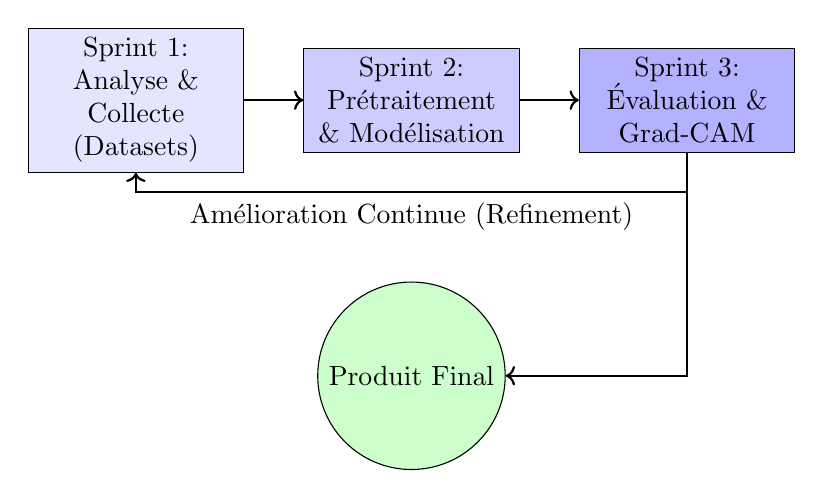
\begin{tikzpicture}[node distance=2cm, auto]
        \node[draw, rectangle, fill=blue!10, text width=2.5cm, align=center] (sprint1) {Sprint 1:\\Analyse \& Collecte (Datasets)};
        \node[draw, rectangle, fill=blue!20, text width=2.5cm, align=center, right of=sprint1, xshift=1.5cm] (sprint2) {Sprint 2:\\Prétraitement \& Modélisation};
        \node[draw, rectangle, fill=blue!30, text width=2.5cm, align=center, right of=sprint2, xshift=1.5cm] (sprint3) {Sprint 3:\\Évaluation \& Grad-CAM};
        
        \draw[thick, ->] (sprint1) -- (sprint2);
        \draw[thick, ->] (sprint2) -- (sprint3);
        \draw[thick, ->] (sprint3.south) |- ++(0,-0.5) -| (sprint1.south) node[pos=0.25, below] {Amélioration Continue (Refinement)};
        
        \node[draw, circle, fill=green!20, below of=sprint2, yshift=-1.5cm] (delivery) {Produit Final};
        \draw[thick, ->] (sprint3) |- (delivery);
    \end{tikzpicture}
    \begin{itemize}
        \item \textbf{Flexibilité :} Adaptation aux contraintes des données médicales.
        \item \textbf{Itérations :} Optimisation progressive des hyperparamètres.
    \end{itemize}
\end{frame}

\begin{frame}{Gestion de Projet --- Tableau des Tâches (PFA)}
    \slidepurpose{Détailler les tâches, leur charge et le type exact de liaison temporelle}{Organisation / planification}
    \textbf{Le tableau ci-dessous affine la planification en ajoutant les décalages et les relations PERT.}
    \centering
    \scriptsize
    \renewcommand{\arraystretch}{1.1}
    \begin{adjustbox}{max width=0.98\textwidth}
    \begin{tabular}{|c|p{5.6cm}|c|p{4.8cm}|}
        \hline
        \textbf{ID} & \textbf{Nom de la Tâche} & \textbf{Durée} & \textbf{Antécédent(s) + liaison} \\ \hline
        \textbf{A} & Cadrage et problématique clinique & 3 j & --- \\ \hline
        \textbf{B} & Analyse SOTA CNN (DenseNet / CheXNet) & 4 j & A (0FD) \\ \hline
        \textbf{C} & Analyse SOTA Swin Transformer / ViT & 4 j & A (0FD) \\ \hline
        \textbf{D} & Étude d'explicabilité XAI et lecture Grad-CAM & 2 j & B (1DD), C (0FF) \\ \hline
        \textbf{E} & Prétraitement $T(X)$, resize et normalisation & 5 j & A (0FD) \\ \hline
        \textbf{F} & Développement de la branche locale CNN & 6 j & B (0FD), E (0FD) \\ \hline
        \textbf{G} & Développement de la branche globale Swin & 7 j & C (0FD), E (0FD) \\ \hline
        \textbf{H} & Intégration du module de gated fusion & 5 j & F (0FD), G (0FD) \\ \hline
        \textbf{I} & Sortie clinique $\Psi$ : score + incertitude & 4 j & H (0FD) \\ \hline
        \textbf{J} & Configuration GPU / Colab / environnement & 2 j & A (1DD) \\ \hline
        \textbf{K} & Entraînement, calibration et optimisation & 10 j & I (0FD), J (0FD) \\ \hline
        \textbf{L} & Évaluation finale, benchmark et métriques & 3 j & K (0FD) \\ \hline
        \textbf{M} & Finalisation rapport, slides et démonstration & 5 j & L (0FD), D (0FD) \\ \hline
    \end{tabular}
    \end{adjustbox}

    \vspace{0.15cm}
    \tiny
    \begin{block}{Lecture de la notation}
        \textbf{Exemple :} \texttt{0FD} signifie \emph{Fin-Début sans décalage}, \texttt{1DD} signifie \emph{Début-Début avec 1 jour de décalage}. 
        La notation générale est : \textbf{[décalage] + [type de liaison]}.
    \end{block}
\end{frame}

\begin{frame}{Gestion de Projet --- Typologie des Dépendances PERT}
    \slidepurpose{Préciser les quatre types de relations temporelles utilisés dans un ordonnancement PERT}{Organisation / planification}
    \scriptsize
    \setlength{\columnsep}{0.7cm}
    \begin{columns}[T,onlytextwidth]
        \begin{column}{0.465\textwidth}
            \begin{block}{FD --- Fin à Début}
                La tâche successeure démarre après la fin de la tâche précédente.\\
                \textbf{Exemple projet :} A $\rightarrow$ B = \texttt{0FD}.
            \end{block}
            \vspace{0.18cm}
            \begin{block}{DD --- Début à Début}
                La tâche successeure peut commencer après le début du précédent, avec un éventuel décalage.\\
                \textbf{Exemple projet :} A $\rightarrow$ J = \texttt{1DD}.
            \end{block}
        \end{column}
        \begin{column}{0.465\textwidth}
            \begin{block}{FF --- Fin à Fin}
                La fin de la tâche successeure est contrainte par la fin d'une autre tâche.\\
                \textbf{Exemple projet :} C $\rightarrow$ D = \texttt{0FF}.
            \end{block}
            \vspace{0.18cm}
            \begin{block}{DF --- Début à Fin}
                Relation plus rare : la fin d'une tâche dépend du début d'une autre.\\
                \textbf{Exemple de notation :} \texttt{2DF}. Elle est documentée dans la méthode, mais non structurante ici.
            \end{block}
        \end{column}
    \end{columns}

    \vspace{0.12cm}
    \begin{alertblock}{Lecture managériale}
        Dans MedFusionNet, la planification repose surtout sur des relations \textbf{FD} pour sécuriser les jalons de validation, avec des liaisons \textbf{DD} et \textbf{FF} pour modéliser les travaux menés en parallèle sans perdre la cohérence globale.
    \end{alertblock}
\end{frame}

% --- FRAME PERT : EXPLICATION ---
\begin{frame}{Méthodologie --- Analyse du Réseau de PERT}
    \slidepurpose{Interpréter les dates, les marges et les zones critiques du planning}{Organisation / planification}
    \scriptsize
    \setlength{\columnsep}{0.75cm}
    \begin{columns}[T,onlytextwidth]
        \begin{column}{0.465\textwidth}
            \begin{block}{Principes de lecture}
                \begin{itemize}
                    \item Le réseau PERT calcule des dates au plus tôt et au plus tard pour chaque activité.
                    \item L'écart entre ces deux positions donne la flexibilité réelle de la tâche.
                    \item Une activité sans marge devient immédiatement sensible à tout retard.
                    \item Les relations \textbf{FD}, \textbf{DD} et \textbf{FF} modifient directement les dates admissibles.
                \end{itemize}
            \end{block}
        \end{column}
        \begin{column}{0.465\textwidth}
            \begin{block}{Lecture des dépendances}
                \begin{itemize}
                    \item \textbf{B} et \textbf{C} sont lancées en parallèle après \textbf{A}.
                    \item \textbf{J} démarre en \textbf{1DD} pour préparer l'infrastructure sans attendre la fin complète du cadrage.
                    \item \textbf{D} démarre tôt, mais se ferme en même temps que \textbf{C} via la contrainte \textbf{0FF}.
                \end{itemize}
            \end{block}
        \end{column}
    \end{columns}
\end{frame}

\begin{frame}{Méthodologie --- Lecture du Chemin Critique}
    \slidepurpose{Mettre en avant les tâches à marge nulle et les points de pilotage du projet}{Organisation / planification}
    \tiny
    \setlength{\columnsep}{0.8cm}
    \begin{columns}[T,onlytextwidth]
        \begin{column}{0.46\textwidth}
            \begin{block}{Interprétation projet}
                \begin{itemize}
                    \item \textbf{H} concentre la convergence des deux branches \textbf{F} et \textbf{G}.
                    \item \textbf{K} attend simultanément la sortie clinique \textbf{I} et l'environnement \textbf{J}.
                    \item \textbf{D} et \textbf{J} restent importantes, mais elles ne pilotent pas la date finale.
                \end{itemize}
            \end{block}
        \end{column}
        \begin{column}{0.46\textwidth}
            \begin{block}{Lecture managériale}
                \begin{itemize}
                    \item Les n{\oe}uds critiques pilotent directement la livraison finale.
                    \item Les tâches quasi critiques, comme \textbf{C} et \textbf{F}, doivent rester sous surveillance.
                    \item Les activités très flexibles, comme \textbf{D} et \textbf{J}, absorbent les aléas sans casser le planning.
                \end{itemize}
            \end{block}
            \vspace{0.16cm}
            \begin{alertblock}{Conséquence managériale}
                Priorité de pilotage : toute dérive sur une tâche à marge nulle décale immédiatement la démonstration finale.
            \end{alertblock}
        \end{column}
    \end{columns}

    \vspace{0.18cm}
    \begin{alertblock}{Chemin critique}
        \textbf{A $\rightarrow$ E $\rightarrow$ G $\rightarrow$ H $\rightarrow$ I $\rightarrow$ K $\rightarrow$ L $\rightarrow$ M}
        \hfill \textbf{Durée totale estimée : 42 jours}
    \end{alertblock}
\end{frame}

\begin{frame}{Gestion de Projet --- Interprétation Opérationnelle}
    \slidepurpose{Transformer le planning théorique en lecture de pilotage concrète pour le projet}{Organisation / planification}
    \scriptsize
    \setlength{\columnsep}{0.8cm}
    \begin{columns}[T,onlytextwidth]
        \begin{column}{0.46\textwidth}
            \begin{block}{Hypothèses de conduite}
                \begin{itemize}
                    \item Le cadrage \textbf{A} alimente rapidement l'état de l'art et le prétraitement pour éviter un démarrage séquentiel trop long.
                    \item Les branches \textbf{F} et \textbf{G} sont parallélisées afin de réduire la durée totale avant l'étape de fusion.
                    \item L'environnement \textbf{J} démarre tôt et l'entraînement \textbf{K} reste le lot le plus long, car il concentre essais, calibration et choix du meilleur checkpoint.
                \end{itemize}
            \end{block}
        \end{column}
        \begin{column}{0.46\textwidth}
            \begin{block}{Lecture de risque}
                \begin{itemize}
                    \item Le verrou principal est la séquence \textbf{E-G-H-I-K}, car elle relie directement données, architecture et validation du modèle.
                    \item Un retard sur \textbf{D} ou \textbf{J} reste absorbable grâce aux marges, alors qu'un retard sur \textbf{H} ou \textbf{K} décale toute la démonstration.
                    \item Les tâches à faible marge, comme \textbf{C} et \textbf{F}, restent à surveiller, tandis que \textbf{L} et \textbf{M} sécurisent la transformation du travail technique en livrables académiques.
                \end{itemize}
            \end{block}
        \end{column}
    \end{columns}

    \vspace{0.16cm}
    \begin{alertblock}{Message clé}
        Le planning montre que la réussite du PFA dépend moins du nombre de tâches que de la bonne maîtrise des quelques étapes critiques qui structurent tout le projet.
    \end{alertblock}
\end{frame}

\begin{frame}{Gestion de Projet --- Tableau des Marges}
    \slidepurpose{Quantifier la flexibilité de chaque tâche à travers la marge libre et la marge totale}{Organisation / planification}
    \centering
    \scriptsize
    \renewcommand{\arraystretch}{1.28}
    \setlength{\tabcolsep}{4.2pt}
    \begin{adjustbox}{max width=0.98\textwidth}
    \begin{tabular}{|c|*{13}{c|}}
        \hline
        \textbf{ID} & \textbf{A} & \textbf{B} & \textbf{C} & \textbf{D} & \textbf{E} & \textbf{F} & \textbf{G} & \textbf{H} & \textbf{I} & \textbf{J} & \textbf{K} & \textbf{L} & \textbf{M} \\ \hline
        \textbf{ML} & 0 & 1 & 0 & 30 & 0 & 1 & 0 & 0 & 0 & 21 & 0 & 0 & 0 \\ \hline
        \textbf{MT} & 0 & 2 & 1 & 30 & 0 & 1 & 0 & 0 & 0 & 21 & 0 & 0 & 0 \\ \hline
    \end{tabular}
    \end{adjustbox}

    \vspace{0.2cm}
    \tiny
    \textbf{ML} = marge libre ; \textbf{MT} = marge totale. Les tâches critiques vérifient \textbf{ML = MT = 0}, tandis que \textbf{D} et \textbf{J} concentrent l'essentiel de la souplesse du planning.
\end{frame}

% --- FRAME PERT : LE SCHÉMA ---
\begin{frame}{Méthodologie --- Schéma du Réseau de PERT}
    \slidepurpose{Visualiser le réseau PERT avec les dates au plus tôt/tard et le chemin critique}{Organisation / planification}
    \tikzsolutionfigure{
    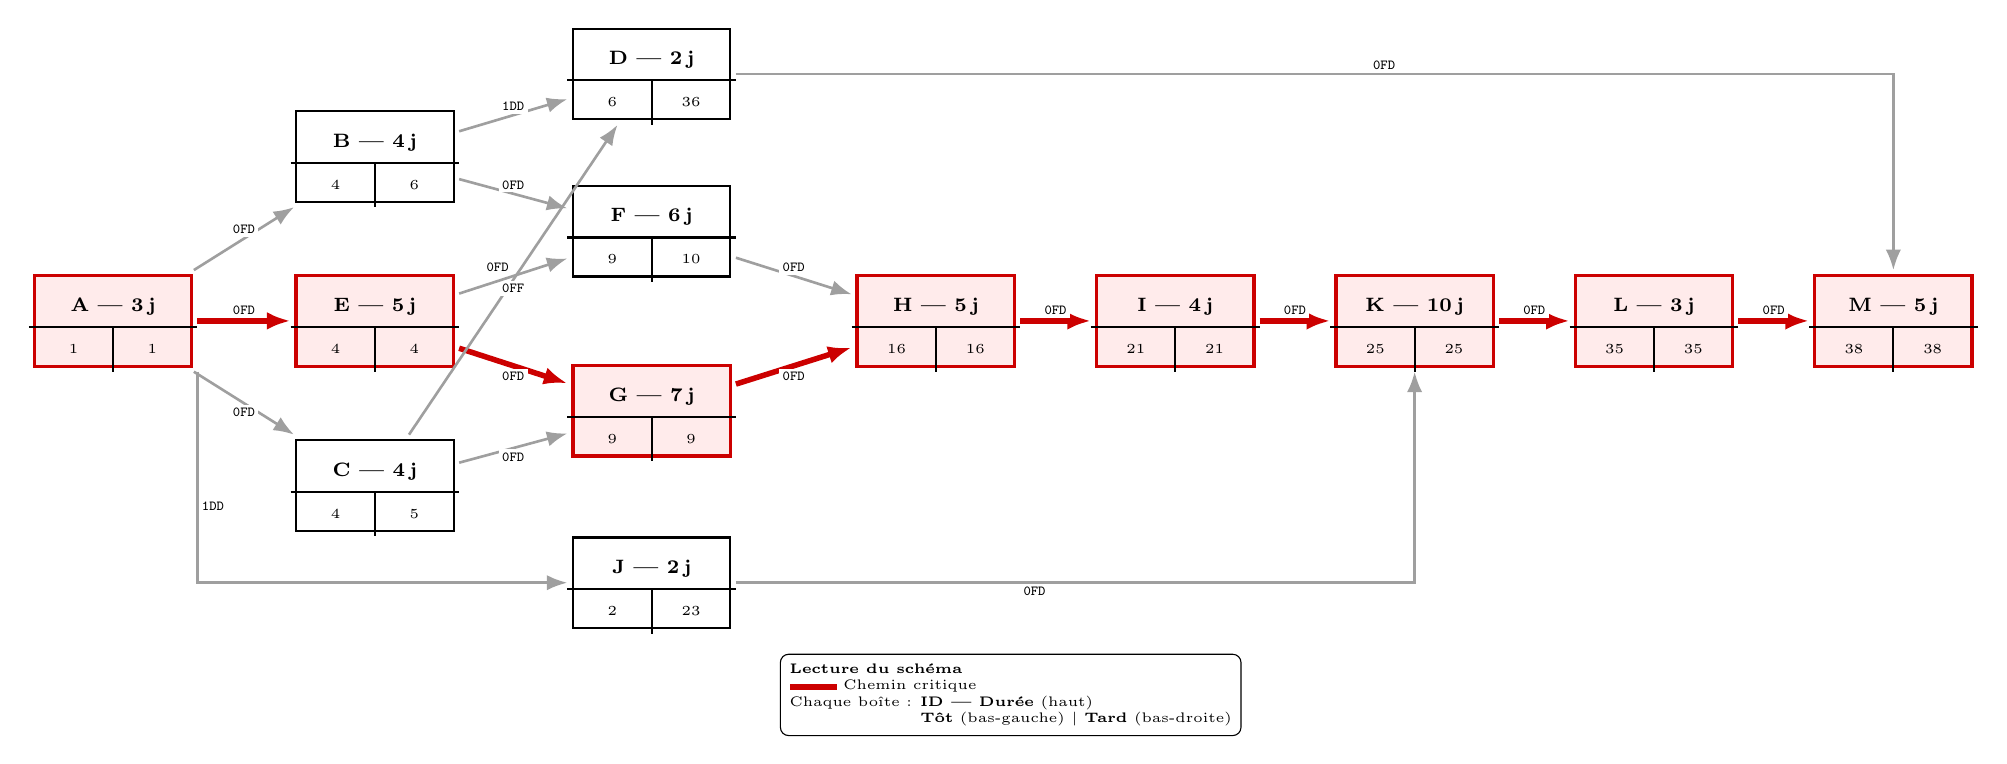
\begin{tikzpicture}[
        x=0.95cm,
        y=0.95cm,
        link/.style={-{Latex[length=2.6mm]}, line width=0.95pt, draw=gray!75},
        clink/.style={-{Latex[length=3mm]}, line width=2pt, draw=red!80!black},
        rel/.style={font=\tiny, fill=white, inner sep=1.2pt}
    ]
        % === NOEUDS PERT (boîtes 3 compartiments) ===
        % \pertnode{nom}{style}{(x,y)}{ID --- durée}{tôt}{tard}
        % Colonne 1
        \pertnode{A}{draw=red!80!black, very thick, fill=red!8}{(0,0)}{A --- 3\,j}{1}{1}
        % Colonne 2
        \pertnode{B}{}{(3.5,2.2)}{B --- 4\,j}{4}{6}
        \pertnode{E}{draw=red!80!black, very thick, fill=red!8}{(3.5,0)}{E --- 5\,j}{4}{4}
        \pertnode{C}{}{(3.5,-2.2)}{C --- 4\,j}{4}{5}
        % Colonne 3
        \pertnode{D}{}{(7.2,3.3)}{D --- 2\,j}{6}{36}
        \pertnode{F}{}{(7.2,1.2)}{F --- 6\,j}{9}{10}
        \pertnode{G}{draw=red!80!black, very thick, fill=red!8}{(7.2,-1.2)}{G --- 7\,j}{9}{9}
        \pertnode{J}{}{(7.2,-3.5)}{J --- 2\,j}{2}{23}
        % Colonne 4--7 (chemin linéaire)
        \pertnode{H}{draw=red!80!black, very thick, fill=red!8}{(11,0)}{H --- 5\,j}{16}{16}
        \pertnode{I}{draw=red!80!black, very thick, fill=red!8}{(14.2,0)}{I --- 4\,j}{21}{21}
        \pertnode{K}{draw=red!80!black, very thick, fill=red!8}{(17.4,0)}{K --- 10\,j}{25}{25}
        \pertnode{L}{draw=red!80!black, very thick, fill=red!8}{(20.6,0)}{L --- 3\,j}{35}{35}
        \pertnode{M}{draw=red!80!black, very thick, fill=red!8}{(23.8,0)}{M --- 5\,j}{38}{38}

        % === LIAISONS CRITIQUES (rouge épais) ===
        \draw[clink] (A) -- node[rel, above] {\texttt{0FD}} (E);
        \draw[clink] (E) -- node[rel, below] {\texttt{0FD}} (G);
        \draw[clink] (G) -- node[rel, below] {\texttt{0FD}} (H);
        \draw[clink] (H) -- node[rel, above] {\texttt{0FD}} (I);
        \draw[clink] (I) -- node[rel, above] {\texttt{0FD}} (K);
        \draw[clink] (K) -- node[rel, above] {\texttt{0FD}} (L);
        \draw[clink] (L) -- node[rel, above] {\texttt{0FD}} (M);

        % === LIAISONS SECONDAIRES (gris) ===
        \draw[link] (A) -- node[rel, above] {\texttt{0FD}} (B);
        \draw[link] (A) -- node[rel, below] {\texttt{0FD}} (C);
        \draw[link] (A.south east) |- node[rel, pos=0.32, right] {\texttt{1DD}} (J.west);
        \draw[link] (B) -- node[rel, above] {\texttt{1DD}} (D);
        \draw[link] (C) -- node[rel, below] {\texttt{0FF}} (D);
        \draw[link] (B) -- node[rel, above] {\texttt{0FD}} (F);
        \draw[link] (E) -- node[rel, above left] {\texttt{0FD}} (F);
        \draw[link] (C) -- node[rel, below] {\texttt{0FD}} (G);
        \draw[link] (F) -- node[rel, above] {\texttt{0FD}} (H);
        \draw[link] (J.east) -| node[rel, pos=0.22, below] {\texttt{0FD}} (K.south);
        \draw[link] (D.east) -| node[rel, pos=0.28, above] {\texttt{0FD}} (M.north);

        % === LÉGENDE ===
        \node[draw, rounded corners=3pt, fill=white, align=left, font=\tiny] at (12,-5) {
            \textbf{Lecture du schéma}\\
            \textcolor{red!80!black}{\rule{0.6cm}{2pt}} Chemin critique\\
            Chaque bo\^ite : \textbf{ID --- Durée} (haut)\\
            \phantom{Chaque bo\^ite : }\textbf{T\^ot} (bas-gauche) \textbar{} \textbf{Tard} (bas-droite)
        };
    \end{tikzpicture}
    }{Réseau PERT de MedFusionNet avec chemin critique et dates au plus tôt / au plus tard.}
\end{frame}

\begin{frame}{Gestion de Projet --- Diagramme de Gantt}
    \slidepurpose{Projeter le planning sur un calendrier opérationnel tout en respectant les liaisons DD, FD et FF}{Organisation / planification}
    \centering
    \small
    \begin{adjustbox}{max width=0.98\textwidth, max totalheight=0.8\textheight}
    \begin{ganttchart}[
        hgrid,
        vgrid,
        x unit=0.222cm,
        y unit chart=0.50cm,
        y unit title=0.45cm,
        title height=1,
        bar height=0.66,
        group height=0.74,
        group peaks tip position=0,
        bar label font=\scriptsize,
        group label font=\scriptsize\bfseries,
        title label font=\scriptsize\bfseries,
        bar label node/.append style={align=left, text width=2.2cm},
        group label node/.append style={align=left},
        bar/.append style={fill=blue!18, draw=blue!70!black},
        group/.append style={fill=black!10, draw=black!65},
        link/.style={-Latex, line width=0.55pt, draw=black!60},
        link label font=\tiny
    ]{1}{42}
        \gantttitle{Calendrier du projet}{42} \\
        \gantttitle{S1}{7}\gantttitle{S2}{7}\gantttitle{S3}{7}\gantttitle{S4}{7}\gantttitle{S5}{7}\gantttitle{S6}{7} \\

        \ganttgroup{Cadrage / études}{1}{8} \\
        \ganttbar[name=A, bar/.append style={fill=red!20, draw=red!75!black}]{A Cadrage}{1}{3} \\
        \ganttbar[name=B]{B SOTA CNN}{4}{7} \\
        \ganttbar[name=C]{C SOTA Swin}{4}{7} \\
        \ganttbar[name=D]{D XAI}{6}{7} \\
        \ganttbar[name=E, bar/.append style={fill=red!20, draw=red!75!black}]{E Prétrait.}{4}{8} \\
        \ganttbar[name=J]{J GPU / Colab}{2}{3} \\

        \ganttgroup{Développement}{9}{24} \\
        \ganttbar[name=F]{F Branche CNN}{9}{14} \\
        \ganttbar[name=G, bar/.append style={fill=red!20, draw=red!75!black}]{G Branche Swin}{9}{15} \\
        \ganttbar[name=H, bar/.append style={fill=red!20, draw=red!75!black}]{H Fusion}{16}{20} \\
        \ganttbar[name=I, bar/.append style={fill=red!20, draw=red!75!black}]{I Sortie clin.}{21}{24} \\

        \ganttgroup{Apprentissage / clôture}{25}{42} \\
        \ganttbar[name=K, bar/.append style={fill=red!20, draw=red!75!black}]{K Entraînt.}{25}{34} \\
        \ganttbar[name=L, bar/.append style={fill=red!20, draw=red!75!black}]{L Évaluat.}{35}{37} \\
        \ganttbar[name=M, bar/.append style={fill=red!20, draw=red!75!black}]{M Rapport / démo}{38}{42} \\

        \ganttlink[link type=f-s, link label=FD]{A}{B}
        \ganttlink[link type=f-s, link label=FD]{A}{C}
        \ganttlink[link type=f-s, link label=FD]{A}{E}
        \ganttlink[link type=s-s, link label=DD+1]{A}{J}
        \ganttlink[link type=s-s, link label=DD+1]{B}{D}
        \ganttlink[link type=f-f, link label=FF]{C}{D}
        \ganttlink[link type=f-s, link label=FD]{B}{F}
        \ganttlink[link type=f-s, link label=FD]{E}{F}
        \ganttlink[link type=f-s, link label=FD]{C}{G}
        \ganttlink[link type=f-s, link label=FD]{E}{G}
        \ganttlink[link type=f-s, link label=FD]{F}{H}
        \ganttlink[link type=f-s, link label=FD]{G}{H}
        \ganttlink[link type=f-s, link label=FD]{H}{I}
        \ganttlink[link type=f-s, link label=FD]{I}{K}
        \ganttlink[link type=f-s, link label=FD]{J}{K}
        \ganttlink[link type=f-s, link label=FD]{K}{L}
        \ganttlink[link type=f-s, link label=FD]{L}{M}
        \ganttlink[link type=f-s, link label=FD]{D}{M}
    \end{ganttchart}
\end{adjustbox}

\end{frame}

% ====================================================================
% PARTIE II --- FAISABILITÉ ENTREPRENEURIALE ET COMMERCIALE
% ====================================================================
\section{Faisabilité Entrepreneuriale}
\subsection{Étude de marché et stratégie}

% --- SLIDE 1 : TITRE DE SECTION ---
\begin{frame}{}
\vfill
\begin{center}
{\Large\bfseries Partie II}\\[0.6em]
{\large Faisabilité Entrepreneuriale et Commerciale}\\[1.2em]
\begin{block}{}
\centering\scriptsize
Démontrer la viabilité économique, le potentiel de marché et la transformation de la solution technique \textbf{MedFusionNet} en un projet d'entreprise viable.
\end{block}
\end{center}
\vfill
\end{frame}

% --- SLIDE 2 : CONTEXTE ET IDENTIFICATION DU PROBLÈME ---
\begin{frame}[t]{Contexte et Identification du Problème}
\slidepurpose{Poser le besoin terrain, l'origine de l'idée et l'avantage concurrentiel de la solution}{Cadrage entrepreneurial}
\scriptsize
\begin{columns}[T,onlytextwidth]
\begin{column}{0.47\textwidth}
\begin{block}{Le Problème}
\begin{itemize}
\setlength{\itemsep}{0.18em}
\item \textbf{Complexité visuelle} des pathologies pulmonaires sur CXR.
\item \textbf{Pénurie mondiale} de radiologues experts (OMS : 1 radiologue / 100\,000 hab. en Afrique).
\item \textbf{Temps d'attente} critiques aux services d'urgence.
\item Les solutions SOTA actuelles restent des \textbf{boîtes noires} non explicables, freinant l'adoption clinique.
\end{itemize}
\end{block}
\end{column}
\begin{column}{0.47\textwidth}
\begin{block}{Origine \& Solution}
\begin{itemize}
\setlength{\itemsep}{0.18em}
\item Observation terrain en \textbf{milieu hospitalier} : besoin réel et non couvert.
\item \textbf{MedFusionNet} apporte un avantage concurrentiel unique :
\begin{itemize}
\setlength{\itemsep}{0.1em}
\item[\textbullet] Double lecture \textbf{locale/globale} (CNN + Swin).
\item[\textbullet] \textbf{Explicabilité} Grad-CAM intégrée.
\item[\textbullet] \textbf{Quantification d'incertitude} (MC-Dropout) pour sécuriser le diagnostic.
\end{itemize}
\end{itemize}
\end{block}
\end{column}
\end{columns}
\begin{alertblock}{Proposition de valeur}
Là où les concurrents fournissent un score opaque, MedFusionNet livre un \textbf{triplet $(p, L^c, u)$} : probabilité, carte explicative et niveau de confiance.
\end{alertblock}
\end{frame}

% --- SLIDE 3 : ÉTUDE DE MARCHÉ & ANALYSES STRATÉGIQUES ---
\begin{frame}[t]{Étude de Faisabilité Commerciale}
\slidepurpose{Synthétiser l'environnement externe et les outils stratégiques SWOT / PESTEL / Porter}{Analyse de marché}
\scriptsize
\begin{columns}[T,onlytextwidth]
\begin{column}{0.47\textwidth}
\begin{block}{Demande identifiée}
\begin{itemize}
\setlength{\itemsep}{0.15em}
\item \textbf{Hôpitaux publics} : réduire les erreurs de diagnostic et optimiser le triage.
\item \textbf{Cliniques privées} : accélérer le flux patients et se différencier.
\item \textbf{Centres de radiologie d'urgence} : aide à la décision 24h/24.
\end{itemize}
\end{block}
\begin{block}{Analyse SWOT (synthèse)}
\renewcommand{\arraystretch}{1.05}
\begin{adjustbox}{max width=\linewidth}
\begin{tabular}{|p{2cm}|p{3.5cm}|}
\hline
\textbf{Forces} & Technologie propriétaire, explicable et quantifiée \\ \hline
\textbf{Faiblesses} & Startup, peu de données cliniques validées \\ \hline
\textbf{Opportunités} & Digitalisation de la santé au Maroc, plan Santé 2025 \\ \hline
\textbf{Menaces} & Réglementation stricte, concurrents internationaux \\ \hline
\end{tabular}
\end{adjustbox}
\end{block}
\end{column}
\begin{column}{0.47\textwidth}
\begin{block}{PESTEL --- Facteurs clés}
\begin{itemize}
\setlength{\itemsep}{0.12em}
\item \textbf{P} : Soutien étatique à l'innovation e-santé.
\item \textbf{E} : Marché IA santé mondial $>$ 45 Mds \$ d'ici 2030.
\item \textbf{S} : Acceptation croissante de l'IA par les praticiens.
\item \textbf{T} : GPU cloud accessibles, frameworks open-source matures.
\item \textbf{E} : Faible empreinte (calcul sur demande).
\item \textbf{L} : Conformité RGPD / Loi 09-08 (protection des données patients).
\end{itemize}
\end{block}
\begin{block}{Porter --- Forces concurrentielles}
\begin{itemize}
\setlength{\itemsep}{0.12em}
\item Barrière à l'entrée élevée (expertise IA + médical).
\item Pouvoir de négociation des hôpitaux : fort $\Rightarrow$ modèle SaaS flexible.
\item Substituts limités : pas d'outil explicable équivalent au Maroc.
\end{itemize}
\end{block}
\end{column}
\end{columns}
\end{frame}

% --- SLIDE 4 : MARKETING STRATÉGIQUE ET MARKETING MIX ---
\begin{frame}[t]{Marketing Stratégique et Marketing Mix}
\slidepurpose{Définir le positionnement STP et le mix marketing 4P pour la commercialisation}{Stratégie marketing}
\scriptsize
\begin{columns}[T,onlytextwidth]
\begin{column}{0.47\textwidth}
\begin{block}{Segmentation \& Positionnement (STP)}
\begin{itemize}
\setlength{\itemsep}{0.15em}
\item \textbf{Segment principal} : Services d'urgence et centres de radiologie à fort flux ($>$50 CXR/jour).
\item \textbf{Segment secondaire} : Plateformes de téléradiologie.
\item \textbf{Ciblage} : B2B, établissements de santé au Maroc puis Afrique francophone.
\item \textbf{Positionnement} : Solution IA \textbf{innovante}, hautement \textbf{fiable} (incertitude quantifiée) et \textbf{transparente} (explicable par Grad-CAM).
\end{itemize}
\end{block}
\end{column}
\begin{column}{0.47\textwidth}
\begin{block}{Marketing Mix --- 4P}
\begin{itemize}
\setlength{\itemsep}{0.15em}
\item \textbf{Produit} : API MedFusionNet + Interface Web intuitive (Streamlit / Gradio). Sortie : $(p, L^c, u)$.
\item \textbf{Prix} : Stratégie de pénétration puis abonnement SaaS par volume de scans (3 paliers).
\item \textbf{Place} : Déploiement Cloud sécurisé (AWS/GCP) ou conteneurisé sur serveur local via Docker.
\item \textbf{Promotion} : Salons technologiques médicaux (GITEX Africa), publications scientifiques, partenariats pilotes avec des CHU.
\end{itemize}
\end{block}
\end{column}
\end{columns}
\begin{alertblock}{Avantage clé}
MedFusionNet se différencie par la \textbf{triple sortie explicable} $(p, L^c, u)$ là où les concurrents ne fournissent qu'un score binaire opaque.
\end{alertblock}
\end{frame}

% --- SLIDE 5 : FAISABILITÉ TECHNIQUE ---
\begin{frame}[t]{Étude de Faisabilité Technique}
\slidepurpose{Valider la viabilité opérationnelle : ressources matérielles et profils humains requis}{Faisabilité technique}
\scriptsize
\begin{columns}[T,onlytextwidth]
\begin{column}{0.47\textwidth}
\begin{block}{Besoins Matériels}
\begin{itemize}
\setlength{\itemsep}{0.15em}
\item \textbf{Calcul} : Serveurs GPU (NVIDIA A100 ou T4) pour l'entraînement et l'inférence temps réel.
\item \textbf{Cloud} : Infrastructure sécurisée (AWS / GCP / Azure) avec chiffrement des données médicales.
\item \textbf{Stockage} : Compatibilité PACS/DICOM pour l'intégration hospitalière native.
\item \textbf{Réseau} : Connexion sécurisée (VPN / TLS) pour la transmission des images.
\end{itemize}
\end{block}
\end{column}
\begin{column}{0.47\textwidth}
\begin{block}{Profils Requis}
\begin{itemize}
\setlength{\itemsep}{0.15em}
\item \textbf{Ingénieur IA / Deep Learning} : Maintenance et amélioration du modèle hybride.
\item \textbf{Développeur Full-Stack} : FastAPI / Streamlit, interface utilisateur et API REST.
\item \textbf{Expert DevOps} : Docker, CI/CD, monitoring et déploiement continu.
\item \textbf{Consultant Radiologue} : Validation clinique, annotation experte et conformité médicale.
\end{itemize}
\end{block}
\end{column}
\end{columns}
\begin{alertblock}{Stack technologique validée}
L'ensemble du pipeline (PyTorch, Flask, Docker) a été \textbf{prototypé et testé} durant le PFA, réduisant significativement le risque technique.
\end{alertblock}
\end{frame}

\subsection{Faisabilité financière et juridique}

% --- SLIDE 6 : ÉTUDE FINANCIÈRE --- BUDGET ET PRÉVISIONS ---
\begin{frame}[t]{Étude Financière --- Budget et Prévisions}
\slidepurpose{Chiffrer l'investissement initial et projeter les revenus sur 12 mois}{Faisabilité financière}
\scriptsize
\begin{columns}[T,onlytextwidth]
\begin{column}{0.52\textwidth}
\begin{block}{Investissement Initial}
\renewcommand{\arraystretch}{1.08}
\begin{adjustbox}{max width=\linewidth}
\begin{tabular}{|p{4.2cm}|r|}
\hline
\textbf{Poste d'investissement} & \textbf{Montant (MAD)} \\ \hline
Développement logiciel (6 mois) & 180\,000 \\ \hline
Infrastructure Cloud / GPU (an 1) & 60\,000 \\ \hline
Licences outils IA \& données & 25\,000 \\ \hline
Marketing de lancement & 35\,000 \\ \hline
Création juridique (SARL) & 8\,000 \\ \hline
Fonds de roulement initial & 42\,000 \\ \hline
\textbf{Total Investissement} & \textbf{350\,000} \\ \hline
\end{tabular}
\end{adjustbox}
\end{block}
\end{column}
\begin{column}{0.44\textwidth}
\begin{block}{Prévisions de Ventes (mois 7--12)}
\renewcommand{\arraystretch}{1.08}
\begin{adjustbox}{max width=\linewidth}
\begin{tabular}{|p{2.6cm}|r|r|}
\hline
\textbf{Segment} & \textbf{Clients} & \textbf{CA/mois} \\ \hline
Cliniques (SaaS) & 5 & 30\,000 \\ \hline
Hôpitaux (licence) & 2 & 40\,000 \\ \hline
Pilotes payants & 3 & 15\,000 \\ \hline
\textbf{Total mensuel} & \textbf{10} & \textbf{85\,000} \\ \hline
\end{tabular}
\end{adjustbox}
\vspace{0.15cm}
\begin{itemize}
\setlength{\itemsep}{0.12em}
\item CA annuel projeté (an 1) : $\sim$510\,000 MAD
\item Objectif an 2 : 20 clients, CA $>$ 1.2M MAD
\end{itemize}
\end{block}
\end{column}
\end{columns}
\begin{alertblock}{Modèle économique}
Revenus récurrents par \textbf{abonnement SaaS} (cliniques) et \textbf{licences annuelles} (hôpitaux), assurant une visibilité financière à moyen terme.
\end{alertblock}
\end{frame}

% --- SLIDE 7 : INDICATEURS DE RENTABILITÉ ---
\begin{frame}[t]{Étude Financière --- Indicateurs de Rentabilité}
\slidepurpose{Calculer les seuils de rentabilité et le BFR pour valider la viabilité économique}{Analyse financière}
\scriptsize
\begin{columns}[T,onlytextwidth]
\begin{column}{0.47\textwidth}
\begin{block}{Charges mensuelles estimées}
\renewcommand{\arraystretch}{1.05}
\begin{adjustbox}{max width=\linewidth}
\begin{tabular}{|p{3.2cm}|r|}
\hline
\textbf{Charges fixes (CF)} & \textbf{MAD/mois} \\ \hline
Salaires (3 ETP) & 36\,000 \\ \hline
Cloud / serveurs GPU & 5\,000 \\ \hline
Locaux / divers & 4\,000 \\ \hline
\textbf{Total CF} & \textbf{45\,000} \\ \hline
\end{tabular}
\end{adjustbox}
\vspace{0.12cm}
\textbf{Charges variables (CV)} : coût API Cloud par scan $\approx$ 0.50 MAD/scan. Pour 10\,000 scans/mois $\Rightarrow$ CV = 5\,000 MAD.
\end{block}
\end{column}
\begin{column}{0.47\textwidth}
\begin{block}{Indicateurs clés}
\begin{itemize}
\setlength{\itemsep}{0.12em}
\item \textbf{Marge brute} :
\[
MB = CA - CV = 85\,000 - 5\,000 = 80\,000
\]
\item \textbf{Taux de marge sur coût variable} :
\[
TMCV = \frac{MB}{CA} = \frac{80\,000}{85\,000} \approx 94,1\%
\]
\item \textbf{Seuil de rentabilité (Point mort)} :
\[
SR = \frac{CF}{TMCV} = \frac{45\,000}{0{,}941} \approx 47\,822~\text{MAD/mois}
\]
\item \textbf{BFR maîtrisé} : paiement SaaS d'avance $\Rightarrow$ BFR faible ($<$ 1 mois de CA).
\end{itemize}
\end{block}
\end{column}
\end{columns}
\begin{alertblock}{Conclusion financière}
Avec un CA mensuel de 85\,000 MAD et un seuil de rentabilité à $\sim$48\,000 MAD, le projet atteint l'\textbf{équilibre dès le 8\textsuperscript{e} mois} d'activité commerciale.
\end{alertblock}
\end{frame}

% --- SLIDE 8 : CADRE JURIDIQUE ET PERSPECTIVES ---
\begin{frame}[t]{Cadre Juridique et Stratégie de Développement}
\slidepurpose{Définir la forme juridique et tracer les axes d'évolution du projet}{Aspects juridiques / perspectives}
\scriptsize
\begin{columns}[T,onlytextwidth]
\begin{column}{0.47\textwidth}
\begin{block}{Forme Juridique --- SARL}
\begin{itemize}
\setlength{\itemsep}{0.15em}
\item \textbf{Choix} : Société à Responsabilité Limitée (SARL).
\item \textbf{Justification} :
\begin{itemize}
\setlength{\itemsep}{0.08em}
\item[\textbullet] Protection du patrimoine des associés fondateurs.
\item[\textbullet] Souplesse de gestion adaptée à une startup tech.
\item[\textbullet] Capital social minimum flexible (1 MAD).
\item[\textbullet] Cadre juridique marocain bien établi pour les SARL.
\end{itemize}
\item \textbf{Conformité} : Loi 09-08 (données personnelles), anonymisation des images médicales, consentement patient.
\end{itemize}
\end{block}
\end{column}
\begin{column}{0.47\textwidth}
\begin{block}{Perspectives de Développement}
\begin{itemize}
\setlength{\itemsep}{0.15em}
\item \textbf{Court terme} : Déploiement pilote dans 2--3 CHU partenaires au Maroc.
\item \textbf{Moyen terme} :
\begin{itemize}
\setlength{\itemsep}{0.08em}
\item[\textbullet] Détection \textbf{multi-pathologies} (Tuberculose, tumeurs, épanchements).
\item[\textbullet] Certification \textbf{dispositif médical} (marquage CE / FDA 510(k)).
\end{itemize}
\item \textbf{Long terme} :
\begin{itemize}
\setlength{\itemsep}{0.08em}
\item[\textbullet] Intégration native dans les logiciels PACS/RIS (compatibilité DICOM universelle).
\item[\textbullet] Expansion vers l'Afrique francophone.
\item[\textbullet] Levée de fonds Série A.
\end{itemize}
\end{itemize}
\end{block}
\end{column}
\end{columns}
\begin{alertblock}{Vision}
De projet académique à \textbf{startup e-health} certifiée : MedFusionNet a le potentiel de devenir un outil de référence pour le diagnostic assisté par IA au Maroc et en Afrique.
\end{alertblock}
\end{frame}
\subsection{Phase 4 — Confiance et explicabilité}
\begin{frame}{Phase 4 — Grad-CAM : schéma de génération}
\slidepurpose{Visualiser le pipeline complet de production d'une heatmap explicative}{Analyse SOTA / évaluation interprétable}
\vspace*{-0.2cm}
\centering
\resizebox{\textwidth}{!}{%
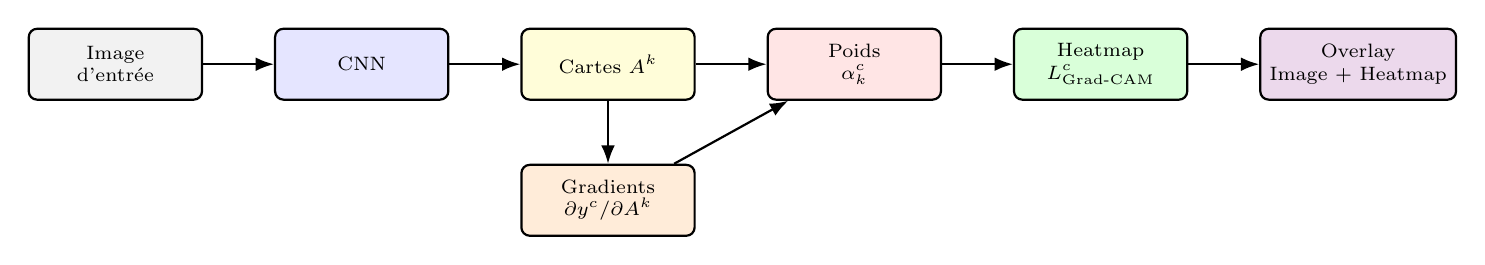
\begin{tikzpicture}[
    >=Latex,
    font=\scriptsize,
    box/.style={draw, rounded corners=3pt, align=center, thick, minimum width=2.2cm, minimum height=0.9cm}
]
\node[box, fill=gray!10] (img) {Image\\d’entrée};
\node[box, fill=blue!10, right=0.9cm of img] (cnn) {CNN};
\node[box, fill=yellow!15, right=0.9cm of cnn] (feat) {Cartes $A^k$};
\node[box, fill=orange!15, below=0.8cm of feat] (grad) {Gradients\\$\partial y^c/\partial A^k$};
\node[box, fill=red!10, right=0.9cm of feat] (weights) {Poids\\$\alpha_k^c$};
\node[box, fill=green!15, right=0.9cm of weights] (heat) {Heatmap\\$L_{\text{Grad-CAM}}^c$};
\node[box, fill=violet!15, right=0.9cm of heat] (overlay) {Overlay\\Image + Heatmap};

\draw[->, thick] (img) -- (cnn);
\draw[->, thick] (cnn) -- (feat);
\draw[->, thick] (feat) -- (weights);
\draw[->, thick] (weights) -- (heat);
\draw[->, thick] (heat) -- (overlay);
\draw[->, thick] (feat) -- (grad);
\draw[->, thick] (grad) -- (weights);
\end{tikzpicture}
}

\vspace{0.12cm}
{\scriptsize
\textbf{Lecture :} l’overlay montre les régions activées associées à la classe prédite.
}
\end{frame}
\section{Solution proposée}
\subsection{Architecture et conception}

\begin{frame}[t]{Solution proposée — Étape 0 : vue d'ensemble}
\slidepurpose{Présenter la logique globale du modèle avant le détail des étapes}{Conception de la solution}
\vspace*{-0.18cm}
\begin{columns}[T,onlytextwidth]
\begin{column}{0.56\textwidth}
\scriptsize
\setlength{\abovedisplayskip}{3pt}
\setlength{\belowdisplayskip}{3pt}
\begin{block}{Principe et formule globale}
MedFusionNet combine deux lectures d'une même radiographie :
\begin{itemize}
\setlength{\itemsep}{0.15em}
\item une branche \textbf{CNN} pour les indices locaux : contours, textures, petites opacités ;
\item une branche \textbf{Swin} pour le contexte global : symétrie thoracique, bilatéralité, cohérence anatomique ;
\item une \textbf{fusion guidée} qui pondère automatiquement les deux branches.
\end{itemize}
\textbf{Chaîne mathématique.}
\[
\begin{aligned}
\tilde X &= T(X)\\
F_c &= \Phi_c(\tilde X), \qquad F_s = \Phi_s(\tilde X)
\end{aligned}
\]
\[
\begin{aligned}
g &= \sigma\!\big(W_g[\mathrm{GAP}(F_c),\mathrm{GAP}(F_s)] + b_g\big)\\
F &= g\odot F_c + (1-g)\odot F_s
\end{aligned}
\]
La sortie finale vérifie \(\Psi(F)=(p,L^c,u)\) : score $p$, heatmap $L^c$, incertitude $u$.
\end{block}
\end{column}
\begin{column}{0.44\textwidth}
\tikzsolutionfigure{%
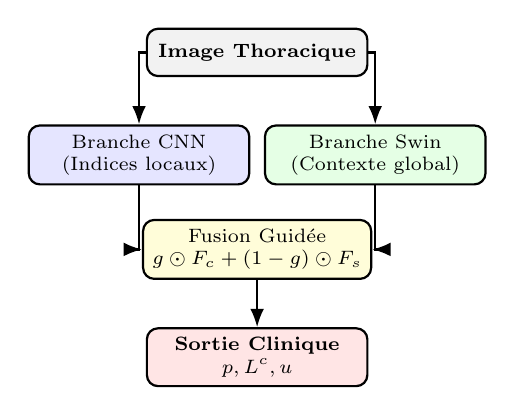
\begin{tikzpicture}[>=Latex, font=\scriptsize, box/.style={draw, rounded corners, thick, fill=white, align=center, minimum width=2.8cm, minimum height=0.6cm}]
\node[box, fill=gray!10] (img) {\textbf{Image Thoracique}};
\node[box, fill=blue!10, below=0.6cm of img, xshift=-1.5cm] (cnn) {Branche CNN\\(Indices locaux)};
\node[box, fill=green!10, below=0.6cm of img, xshift=1.5cm] (swin) {Branche Swin\\(Contexte global)};
\node[box, fill=yellow!15, below=1.8cm of img] (fusion) {Fusion Guidée\\$g\odot F_c + (1-g)\odot F_s$};
\node[box, fill=red!10, below=0.6cm of fusion] (out) {\textbf{Sortie Clinique}\\$p, L^c, u$};
\draw[->, thick] (img) -| (cnn);
\draw[->, thick] (img) -| (swin);
\draw[->, thick] (cnn) |- (fusion);
\draw[->, thick] (swin) |- (fusion);
\draw[->, thick] (fusion) -- (out);
\end{tikzpicture}%
}{Vue d'ensemble du pipeline complet}
\end{column}
\end{columns}
\end{frame}

\subsection{Pipeline détaillé}

\begin{frame}[t]{Solution proposée — Étape 1 : échantillon d'entrée}
\slidepurpose{Définir la donnée d'entrée et ce qu'elle contient avant tout calcul}{Conception détaillée}
\vspace*{-0.18cm}
\begin{columns}[T,onlytextwidth]
\begin{column}{0.56\textwidth}
\scriptsize
\setlength{\abovedisplayskip}{3pt}
\setlength{\belowdisplayskip}{3pt}
\begin{block}{Image et variabilité}
Une radiographie thoracique est modélisée par :
\[
X\in\mathbb{R}^{H\times W}
\]
\noindent avec une étiquette binaire :
\[
\begin{cases}
y=1 & \text{pneumonie}\\
y=0 & \text{normal ou autre classe négative}
\end{cases}
\]
\textbf{Pourquoi l'entrée est difficile.}
L'image brute contient à la fois le signal clinique et des facteurs parasites :
\begin{itemize}
\setlength{\itemsep}{0.15em}
\item variations d'intensité et de contraste selon l'appareil ;
\item bruit, annotations, câbles et autres artefacts ;
\item cadrage, résolution et structures normales parfois trompeuses.
\end{itemize}
\textbf{Exemple :} deux clichés de même classe peuvent avoir un contraste ou un centrage très différents ; le modèle doit ignorer cette variabilité non pathologique.
\end{block}
\end{column}
\begin{column}{0.44\textwidth}
\tikzsolutionfigure{%
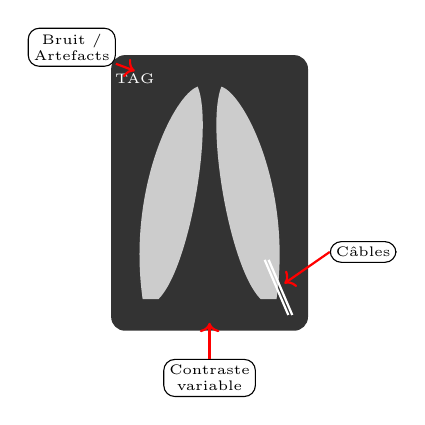
\begin{tikzpicture}[font=\scriptsize]
\draw[draw=none, fill=black!80, rounded corners=5pt] (0,0) rectangle (2.5,3.5);
\draw[draw=none, fill=gray!40] (0.4, 0.4) .. controls (0.2, 1.8) and (0.8, 3) .. (1.1, 3.1) .. controls (1.3, 2.6) and (1.0, 0.8) .. (0.6, 0.4) -- cycle;
\draw[draw=none, fill=gray!40] (2.1, 0.4) .. controls (2.3, 1.8) and (1.7, 3) .. (1.4, 3.1) .. controls (1.2, 2.6) and (1.5, 0.8) .. (1.9, 0.4) -- cycle;
\node[text=white, font=\tiny] at (0.3, 3.2) {TAG};
\draw[white, thick] (2.3,0.2) -- (2.0, 0.9);
\draw[white, thick] (2.25,0.2) -- (1.95, 0.9);
\node[draw, fill=white, rounded corners, inner sep=2pt, font=\tiny, align=center] (bruit) at (-0.5, 3.6) {Bruit /\\Artefacts};
\draw[->, thick, red] (bruit) -- (0.3, 3.3);
\node[draw, fill=white, rounded corners, inner sep=2pt, font=\tiny, align=center] (cable) at (3.2, 1) {Câbles};
\draw[->, thick, red] (cable.west) -- (2.2, 0.6);
\node[draw, fill=white, rounded corners, inner sep=2pt, font=\tiny, align=center] (contrast) at (1.25, -0.6) {Contraste\\variable};
\draw[->, thick, red] (contrast) -- (1.25, 0.1);
\end{tikzpicture}%
}{Échantillon brut provenant du dataset}
\end{column}
\end{columns}
\end{frame}

\begin{frame}[t]{Solution proposée — Étape 2 : prétraitement}
\slidepurpose{Standardiser l'image avant son entrée dans les deux branches du modèle}{Développement / préparation des données}
\vspace*{-0.18cm}
\begin{columns}[T,onlytextwidth]
\begin{column}{0.56\textwidth}
\scriptsize
\setlength{\abovedisplayskip}{3pt}
\setlength{\belowdisplayskip}{3pt}
\begin{block}{Transformation}
Le prétraitement applique une chaîne de standardisation :
\[
\tilde X=T(X)=A\big(R(N(X))\big)
\]
\noindent où $N$ normalise les intensités, $R$ redimensionne et $A$ peut améliorer localement le contraste.
\end{block}
\begin{block}{Ce que la donnée devient}
\[
\text{normalisation :}\qquad X_{norm}=\frac{X-\mu}{\sigma}
\]
\[
\begin{aligned}
\text{redimensionnement :}\qquad
X&\in\mathbb{R}^{H\times W}\\
&\longrightarrow \tilde X\in\mathbb{R}^{H_0\times W_0}
\end{aligned}
\]
\textbf{Exemple :} $1024\times1024 \rightarrow 384\times384$. Cette étape réduit le coût mémoire, homogénéise les entrées et diminue le risque que le modèle prenne une différence d'acquisition pour une pneumonie.
\end{block}
\end{column}
\begin{column}{0.44\textwidth}
\tikzsolutionfigure{%
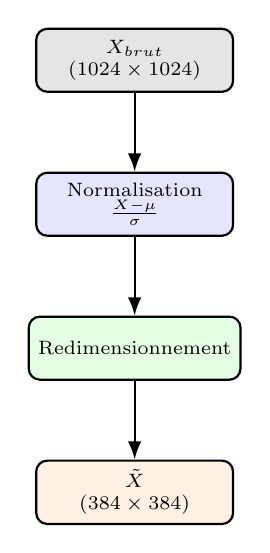
\begin{tikzpicture}[>=Latex, font=\scriptsize, box/.style={draw, thick, rounded corners, fill=white, align=center, minimum width=2.5cm, minimum height=0.8cm}]
\node[box, fill=gray!20] (brut) {$X_{brut}$\\($1024 \times 1024$)};
\node[box, fill=blue!10, below=1cm of brut] (norm) {Normalisation\\$\frac{X - \mu}{\sigma}$};
\node[box, fill=green!10, below=1cm of norm] (resize) {Redimensionnement};
\node[box, fill=orange!10, below=1cm of resize] (final) {$\tilde{X}$\\($384 \times 384$)};
\draw[->, thick] (brut) -- (norm);
\draw[->, thick] (norm) -- (resize);
\draw[->, thick] (resize) -- (final);
\end{tikzpicture}%
}{Image après normalisation et redimensionnement}
\end{column}
\end{columns}
\end{frame}

\begin{frame}[t]{Solution proposée — Étape 3 : branche CNN locale}
\slidepurpose{Extraire les motifs fins et localisés par une lecture convolutive}{Modélisation de la branche locale}
\vspace*{-0.18cm}
\begin{columns}[T,onlytextwidth]
\begin{column}{0.56\textwidth}
\scriptsize
\setlength{\abovedisplayskip}{3pt}
\setlength{\belowdisplayskip}{3pt}
\begin{block}{Lecture locale par CNN}
La branche locale produit :
\[
F_c=\Phi_c(\tilde X)\in\mathbb{R}^{H'\times W'\times C_c}
\]
\noindent Une convolution applique un filtre sur un voisinage restreint :
\[
F^{(\ell)}_{i,j,c'}=\sum_{u,v,c}W^{(\ell)}_{u,v,c,c'}\,F^{(\ell-1)}_{i+u,j+v,c}+b^{(\ell)}_{c'}
\]
\textbf{Ce que la branche voit réellement.}
\begin{itemize}
\setlength{\itemsep}{0.15em}
\item bords pleuraux, côtes, contours pulmonaires ;
\item textures diffuses ou focales ;
\item petites consolidations et opacités locales ;
\item transitions fines entre tissu sain et tissu suspect.
\end{itemize}
\textbf{Exemple :} une opacité basale discrète peut être amplifiée par la comparaison locale entre intensités voisines.
\end{block}
\end{column}
\begin{column}{0.44\textwidth}
\tikzsolutionfigure{%
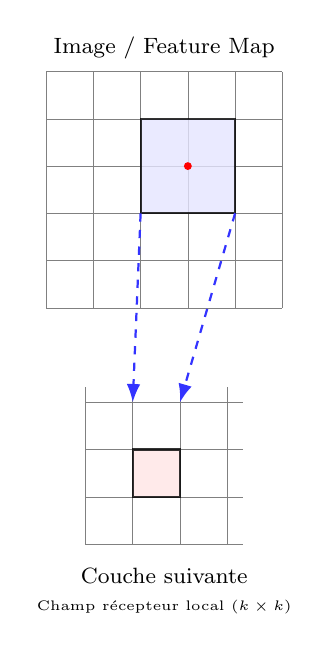
\begin{tikzpicture}[>=Latex, font=\scriptsize]
\draw[step=0.6cm, gray, very thin] (0,0) grid (3,3);
\draw[thick, fill=blue!10, opacity=0.8] (1.2,1.2) rectangle (2.4,2.4);
\node[font=\footnotesize, align=center] at (1.5, 3.3) {Image / Feature Map};
\begin{scope}[yshift=-3cm, xshift=0.5cm]
\draw[step=0.6cm, gray, very thin] (0,0) grid (2,2);
\draw[thick, fill=red!10, opacity=0.8] (0.6,0.6) rectangle (1.2,1.2);
\node[font=\footnotesize, align=center] at (1, -0.4) {Couche suivante};
\end{scope}
\draw[->, thick, dashed, draw=blue!80] (1.2, 1.2) -- (1.1, -1.2);
\draw[->, thick, dashed, draw=blue!80] (2.4, 1.2) -- (1.7, -1.2);
\fill[red] (1.8, 1.8) circle (0.05);
\node[draw=none, fill=none, font=\tiny] at (1.5, -3.8) {Champ récepteur local ($k \times k$)};
\end{tikzpicture}%
}{Représentation locale extraite par la branche CNN}
\end{column}
\end{columns}
\end{frame}

\begin{frame}[t]{Solution proposée — Étape 4 : branche Swin globale}
\slidepurpose{Extraire une représentation de contexte capable de relier des régions éloignées}{Modélisation de la branche globale}
\vspace*{-0.18cm}
\begin{columns}[T,onlytextwidth]
\begin{column}{0.56\textwidth}
\scriptsize
\setlength{\abovedisplayskip}{3pt}
\setlength{\belowdisplayskip}{3pt}
\begin{block}{Lecture globale par Swin}
L'image prétraitée est découpée en patches puis projetée :
\[
z_i = E\,x_i + e_i^{pos}
\]
\noindent La branche globale calcule ensuite :
\[
F_s=\Phi_s(\tilde X)\in\mathbb{R}^{H'\times W'\times C_s}
\]
\[
Q=XW_Q,\quad K=XW_K,\quad V=XW_V
\]
\[
\mathrm{Attention}(Q,K,V)=\mathrm{softmax}\!\left(\frac{QK^\top}{\sqrt{d_k}}\right)V
\]
Dans Swin, cette attention est calculée par fenêtres, puis les fenêtres sont décalées pour reconnecter les régions voisines.
\textbf{Ce que la branche globale apporte.}
Elle relie des zones éloignées : apex, bases, hémithorax droit/gauche, médiastin. Si une anomalie n'a de sens que par sa \textbf{distribution spatiale}, Swin la capture mieux qu'un CNN purement local.
\end{block}
\end{column}
\begin{column}{0.44\textwidth}
\tikzsolutionfigure{%
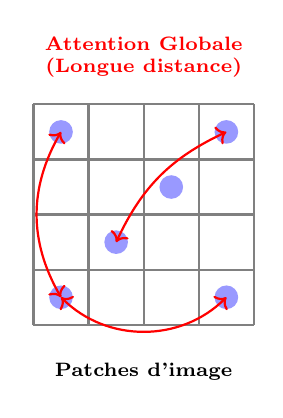
\begin{tikzpicture}[font=\scriptsize]
\draw[step=0.7cm, gray, thick] (0,0) grid (2.8, 2.8);
\foreach \x/\y in {0.35/0.35, 0.35/2.45, 2.45/0.35, 2.45/2.45, 1.05/1.05, 1.75/1.75} {
    \fill[blue!40] (\x,\y) circle (0.15);
}
\draw[<->, thick, red] (0.35, 0.35) to[bend right=45] (2.45, 0.35);
\draw[<->, thick, red] (0.35, 0.35) to[bend left=30] (0.35, 2.45);
\draw[<->, thick, red] (1.05, 1.05) to[bend left=20] (2.45, 2.45);
\node[draw=none, fill=none, font=\scriptsize, align=center] at (1.4, -0.6) {\textbf{Patches d'image}};
\node[draw=none, fill=none, font=\scriptsize, text=red, align=center] at (1.4, 3.4) {\textbf{Attention Globale}\\\textbf{(Longue distance)}};
\end{tikzpicture}%
}{Représentation globale extraite par la branche Swin}
\end{column}
\end{columns}
\end{frame}

\begin{frame}[t]{Solution proposée — Étape 5 : fusion guidée}
\slidepurpose{Combiner les indices locaux et globaux sans imposer un poids fixe à chaque branche}{Conception du coeur de fusion}
\vspace*{-0.18cm}
\begin{columns}[T,onlytextwidth]
\begin{column}{0.56\textwidth}
\scriptsize
\setlength{\abovedisplayskip}{3pt}
\setlength{\belowdisplayskip}{3pt}
\begin{block}{Porte de fusion et interprétation}
On résume d'abord chaque branche par un vecteur global :
\[
\bar F_c=\mathrm{GAP}(F_c),\qquad \bar F_s=\mathrm{GAP}(F_s)
\]
\noindent Puis on apprend un coefficient de fusion :
\[
g=\sigma\!\left(W_g[\bar F_c,\bar F_s]+b_g\right)
\]
\[
F = g\odot F_c + (1-g)\odot F_s
\]
Si $g\approx 1$, le modèle privilégie l'indice local ; si $g\approx 0$, il privilégie le contexte global.
\textbf{Exemples.}
\textbf{Exemple 1 :} foyer net et compact $\Rightarrow g\approx 0.8$.\\
\textbf{Exemple 2 :} atteinte diffuse ou bilatérale $\Rightarrow g\approx 0.3$.\\[0.15em]
La fusion n'est donc pas une moyenne fixe : elle s'adapte à la structure réelle de l'image.
\end{block}
\end{column}
\begin{column}{0.44\textwidth}
\tikzsolutionfigure{%
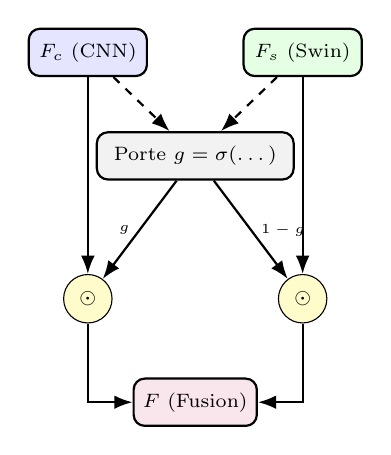
\begin{tikzpicture}[>=Latex, font=\scriptsize, box/.style={draw, rounded corners, thick, fill=white, align=center, minimum width=1.5cm, minimum height=0.6cm}]
\node[box, fill=blue!10] (fc) {$F_c$ (CNN)};
\node[box, fill=green!10, right=1.2cm of fc] (fs) {$F_s$ (Swin)};
\node[box, fill=gray!10, align=center, minimum width=2.5cm, below=1cm of $(fc)!0.5!(fs)$] (gate) {Porte $g = \sigma(\dots)$};
\node[draw, circle, fill=yellow!20, below=2.5cm of fc] (mul_c) {$\odot$};
\node[draw, circle, fill=yellow!20, below=2.5cm of fs] (mul_s) {$\odot$};
\node[box, fill=purple!10, below=1cm of $(mul_c)!0.5!(mul_s)$] (f) {$F$ (Fusion)};
\draw[->, thick] (fc) -- (mul_c);
\draw[->, thick] (fs) -- (mul_s);
\draw[->, thick, dashed] (fc) -- (gate);
\draw[->, thick, dashed] (fs) -- (gate);
\draw[->, thick] (gate) -- node[left, font=\tiny] {$g$} (mul_c);
\draw[->, thick] (gate) -- node[right, font=\tiny] {$1-g$} (mul_s);
\draw[->, thick] (mul_c) |- (f);
\draw[->, thick] (mul_s) |- (f);
\end{tikzpicture}%
}{Fusion adaptative entre la branche locale et la branche globale}
\end{column}
\end{columns}
\end{frame}

\begin{frame}[t]{Solution proposée — Étape 6 : classification}
\slidepurpose{Transformer la représentation fusionnée en probabilité de pneumonie}{Tête de décision}
\vspace*{-0.18cm}
\begin{columns}[T,onlytextwidth]
\begin{column}{0.56\textwidth}
\scriptsize
\setlength{\abovedisplayskip}{3pt}
\setlength{\belowdisplayskip}{3pt}
\begin{block}{Score de classe}
La représentation fusionnée est condensée en un vecteur :
\[
z=\mathrm{GAP}(F)
\]
\noindent puis convertie en probabilité :
\[
p(y=1|X)=\sigma(w^\top z+b)
\]
\end{block}
\begin{block}{Décision pratique}
Avec un seuil $\tau$ :
\[
\hat y =
\begin{cases}
1 & \text{si } p(y=1|X)\ge \tau\\
0 & \text{sinon}
\end{cases}
\]
\textbf{Exemple :} si $p=0.91$ et $\tau=0.5$, la prédiction est positive avec une forte marge. Si $p=0.54$, la décision reste positive mais devient fragile : elle doit être lue avec la heatmap et l'incertitude.
\end{block}
\end{column}
\begin{column}{0.44\textwidth}
\tikzsolutionfigure{%
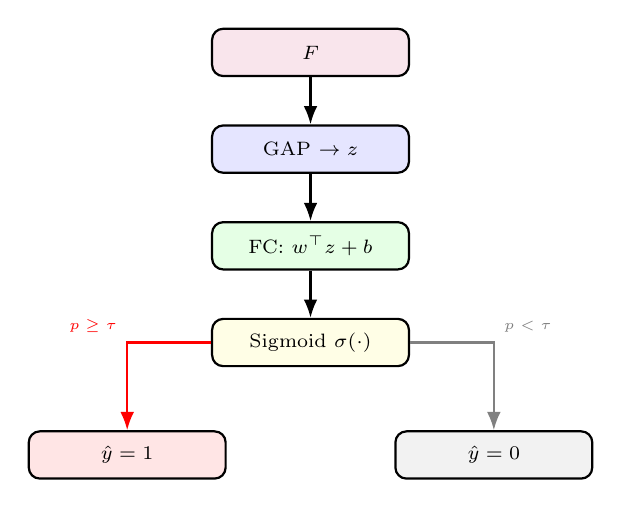
\begin{tikzpicture}[>=Latex, font=\scriptsize, box/.style={draw, rounded corners, thick, fill=white, align=center, minimum width=2.5cm, minimum height=0.6cm}]
\node[box, fill=purple!10] (f) {$F$};
\node[box, fill=blue!10, below=0.6cm of f] (gap) {GAP $\rightarrow z$};
\node[box, fill=green!10, below=0.6cm of gap] (fc) {FC: $w^\top z + b$};
\node[box, fill=yellow!10, below=0.6cm of fc] (sig) {Sigmoid $\sigma(\cdot)$};
\node[box, fill=red!10, below left=0.8cm and -0.2cm of sig] (out1) {$\hat{y}=1$};
\node[box, fill=gray!10, below right=0.8cm and -0.2cm of sig] (out0) {$\hat{y}=0$};
\draw[->, thick] (f) -- (gap);
\draw[->, thick] (gap) -- (fc);
\draw[->, thick] (fc) -- (sig);
\draw[->, thick, red] (sig) -| node[above left, font=\tiny] {$p \ge \tau$} (out1);
\draw[->, thick, gray] (sig) -| node[above right, font=\tiny] {$p < \tau$} (out0);
\end{tikzpicture}%
}{Passage de la représentation fusionnée au score de classe}
\end{column}
\end{columns}
\end{frame}

\begin{frame}[t]{Solution proposée — Étape 7 : localisation et incertitude}
\slidepurpose{Produire une explication spatiale et mesurer la fiabilité de la décision}{Sorties interprétables}
\vspace*{-0.18cm}
\begin{columns}[T,onlytextwidth]
\begin{column}{0.56\textwidth}
\footnotesize
\setlength{\abovedisplayskip}{3pt}
\setlength{\belowdisplayskip}{3pt}
\begin{block}{Localisation et incertitude}
À partir des cartes finales $A^k$ :
\[
\alpha_k^c=\frac{1}{Z}\sum_i\sum_j \frac{\partial y^c}{\partial A^k_{ij}}
\]
\[
L^c=\mathrm{ReLU}\!\left(\sum_k \alpha_k^c A^k\right)
\]
La heatmap montre \textbf{où} le modèle a trouvé des indices pour la classe prédite.
\textbf{Incertitude.}
En répétant plusieurs passes avec dropout actif :
\[
u=\mathrm{Var}_t(p_t)
\]
\textbf{Exemple :} si $p_t=\{0.87,0.88,0.89\}$, la variance est faible ; si $p_t=\{0.42,0.81,0.57\}$, la décision est instable et doit être relue.
\end{block}
\end{column}
\begin{column}{0.44\textwidth}
\tikzsolutionfigure{%
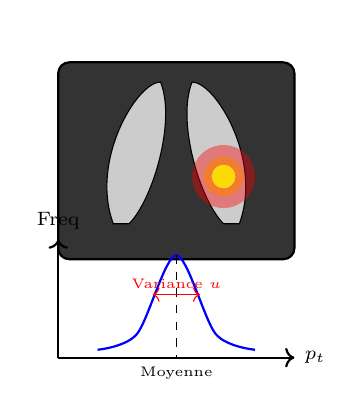
\begin{tikzpicture}[font=\scriptsize]
\node[draw, thick, rounded corners, minimum width=3cm, minimum height=2.5cm, fill=black!80] (bg) at (0, 2) {};
\draw[fill=gray!40] (-0.8, 1.2) .. controls (-1.1, 2) and (-0.5, 3) .. (-0.2, 3) .. controls (0, 2.5) and (-0.3, 1.5) .. (-0.6, 1.2) -- cycle;
\draw[fill=gray!40] (0.8, 1.2) .. controls (1.1, 2) and (0.5, 3) .. (0.2, 3) .. controls (0, 2.5) and (0.3, 1.5) .. (0.6, 1.2) -- cycle;
\fill[red, opacity=0.4] (0.6, 1.8) circle (0.4);
\fill[orange, opacity=0.6] (0.6, 1.8) circle (0.25);
\fill[yellow, opacity=0.8] (0.6, 1.8) circle (0.15);
\node[text=white, font=\tiny, align=center] at (0, 3.5) {\textbf{Grad-CAM $L^c$}};
\draw[->, thick] (-1.5, -0.5) -- (1.5, -0.5) node[right] {$p_t$};
\draw[->, thick] (-1.5, -0.5) -- (-1.5, 1) node[above] {Freq};
\draw[thick, blue] plot[smooth] coordinates {(-1.0, -0.4) (-0.5, -0.2) (0, 0.8) (0.5, -0.2) (1.0, -0.4)};
\draw[dashed] (0, 0.8) -- (0, -0.5) node[below] {\tiny Moyenne};
\draw[<->, red] (-0.3, 0.3) -- (0.3, 0.3) node[midway, above=-0.05cm] {\tiny Variance $u$};
\end{tikzpicture}%
}{Heatmap explicative et estimation d'incertitude}
\end{column}
\end{columns}
\end{frame}

\begin{frame}[t]{Solution proposée — Étape 8 : apprentissage}
\slidepurpose{Définir exactement ce qui est optimisé pendant l'entraînement}{Développement / entraînement}
\vspace*{-0.18cm}
\begin{columns}[T,onlytextwidth]
\begin{column}{0.56\textwidth}
\footnotesize
\setlength{\abovedisplayskip}{3pt}
\setlength{\belowdisplayskip}{3pt}
\begin{block}{Fonction objectif}
\[
\mathcal{L}=
\mathcal{L}_{cls}
\;+\;
\lambda_1\mathcal{L}_{loc}
\;+\;
\lambda_2\mathcal{L}_{cons}
\;+\;
\lambda_3\mathcal{L}_{cal}
\]
\end{block}
\begin{block}{Sens de chaque terme}
\defitem{$\mathcal{L}_{cls}$}{apprendre la bonne classe.}
\defitem{$\mathcal{L}_{loc}$}{contraindre la heatmap à rester cliniquement plausible.}
\defitem{$\mathcal{L}_{cons}$}{garder une prédiction stable sous augmentation.}
\defitem{$\mathcal{L}_{cal}$}{mieux aligner confiance prédite et fréquence réelle d'erreur.}
\textbf{Exemple :} sur un dataset déséquilibré, $\mathcal{L}_{cls}$ peut être une Focal Loss afin de mieux traiter les cas rares ou difficiles.
\end{block}
\end{column}
\begin{column}{0.44\textwidth}
\tikzsolutionfigure{%
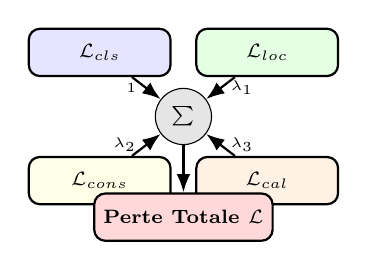
\begin{tikzpicture}[>=Latex, font=\scriptsize, box/.style={draw, rounded corners, thick, fill=white, align=center, minimum width=1.8cm, minimum height=0.6cm}]
\node[box, fill=blue!10] (cls) {$\mathcal{L}_{cls}$};
\node[box, fill=green!10, right=0.3cm of cls] (loc) {$\mathcal{L}_{loc}$};
\node[box, fill=yellow!10, below=1cm of cls] (cons) {$\mathcal{L}_{cons}$};
\node[box, fill=orange!10, below=1cm of loc] (cal) {$\mathcal{L}_{cal}$};
\node[draw, circle, fill=gray!20] at ($(cls)!0.5!(cal)$) (sum) {$\sum$};
\node[box, fill=red!15, below=0.6cm of sum] (total) {\textbf{Perte Totale $\mathcal{L}$}};
\draw[->, thick] (cls) -- node[left, font=\tiny] {$1$} (sum);
\draw[->, thick] (loc) -- node[right, font=\tiny] {$\lambda_1$} (sum);
\draw[->, thick] (cons) -- node[left, font=\tiny] {$\lambda_2$} (sum);
\draw[->, thick] (cal) -- node[right, font=\tiny] {$\lambda_3$} (sum);
\draw[->, thick] (sum) -- (total);
\end{tikzpicture}%
}{Schéma de la perte totale et de ses composantes}
\end{column}
\end{columns}
\end{frame}

\begin{frame}[t]{Solution proposée — Étape 9 : sortie clinique}
\slidepurpose{Montrer comment les sorties du modèle deviennent une aide concrète pour le workflow médical}{Validation métier / déploiement}
\vspace*{-0.18cm}
\begin{columns}[T,onlytextwidth]
\begin{column}{0.56\textwidth}
\footnotesize
\setlength{\abovedisplayskip}{3pt}
\setlength{\belowdisplayskip}{3pt}
\begin{block}{Sortie exploitable pour le clinicien}
Pour une image $X$, le modèle renvoie :
\[
\big(p(y=1|X),\,L^c,\,u\big)
\]
soit un score de pneumonie, une heatmap explicative et une estimation d'incertitude.
\textbf{Comment cela aide le clinicien.}
\begin{itemize}
\setlength{\itemsep}{0.15em}
\item score élevé + faible incertitude : cas à prioriser ;
\item score modéré + incertitude élevée : revue humaine prioritaire ;
\item score faible + faible incertitude : cas probablement normal.
\end{itemize}
\textbf{Limite :} une heatmap plausible reste un support de lecture, pas une preuve diagnostique.
\end{block}
\end{column}
\begin{column}{0.44\textwidth}
\tikzsolutionfigure{%
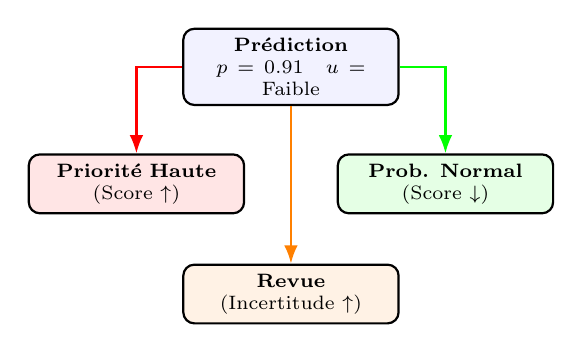
\begin{tikzpicture}[>=Latex, font=\scriptsize, box/.style={draw, rounded corners, thick, fill=white, align=center, text width=2.5cm}]
\node[box, fill=blue!05] (pred) {\textbf{Prédiction}\\$p=0.91 \quad u=\text{Faible}$};
\node[box, fill=red!10, below left=0.6cm and -0.8cm of pred] (high) {\textbf{Priorité Haute}\\(Score $\uparrow$)};
\node[box, fill=green!10, below right=0.6cm and -0.8cm of pred] (low) {\textbf{Prob. Normal}\\(Score $\downarrow$)};
\node[box, fill=orange!10, below=2cm of pred] (rev) {\textbf{Revue}\\(Incertitude $\uparrow$)};
\draw[->, thick, draw=red] (pred) -| (high);
\draw[->, thick, draw=green] (pred) -| (low);
\draw[->, thick, draw=orange] (pred) -- (rev);
\end{tikzpicture}%
}{Sortie finale utilisable par le clinicien}
\end{column}
\end{columns}
\end{frame}
\subsection{Implémentation et Outils techniques}
\begin{frame}[t]{Implémentation — Dataset Chest X-Ray}
\slidepurpose{Justifier la sélection et les caractéristiques des données d'apprentissage}{Préparation des données}
\vspace*{-0.18cm}
\begin{columns}[T,onlytextwidth]
\begin{column}{0.56\textwidth}
\scriptsize
\setlength{\abovedisplayskip}{2pt}
\setlength{\belowdisplayskip}{2pt}
\begin{block}{Spécifications \& Accès aux données}
Dataset Kaggle de Paul Mooney (5\,856 images).
\begin{itemize}
\setlength{\itemsep}{0.05em}
\item \textbf{Classes} : \textit{NORMAL} vs \textit{PNEUMONIA}.
\item \textbf{Défi} : Déséquilibre fort (plus de cas malades).
\item \textbf{Choix} : Utilisation de la \textit{Focal Loss} pour corriger le biais de majorité et focaliser sur les cas difficiles.
\end{itemize}
\vspace{0.3cm}
\centering
\begin{tikzpicture}[font=\tiny]
\node[inner sep=0pt] (qr) {\href{https://www.kaggle.com/paultimothymooney/chest-xray-pneumonia}{
\includegraphics[width=3cm]{kaggle_qr.png}}};
\node[right=0.2cm of qr, text width=4.5cm, align=left] {
\href{https://www.kaggle.com/paultimothymooney/chest-xray-pneumonia}{\textbf{\color{blue}Lien Kaggle :} \\ \scriptsize (Scanner pour accéder \\ au dataset)}
};
\end{tikzpicture}
\end{block}
\end{column}
\begin{column}{0.44\textwidth}
\tikzsolutionfigure{%
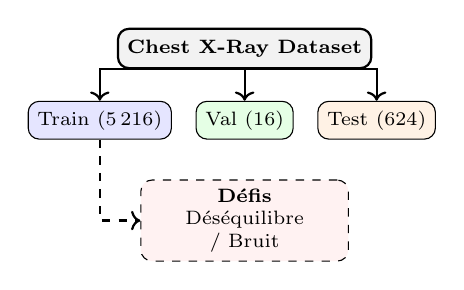
\begin{tikzpicture}[font=\scriptsize, align=center]
\node[draw, rounded corners, thick, fill=gray!10, minimum width=3cm, minimum height=0.5cm] (dataset) {\textbf{Chest X-Ray Dataset}};
\node[draw, rounded corners, fill=blue!10, below left=0.4cm and -0.7cm of dataset] (train) {Train (5\,216)};
\node[draw, rounded corners, fill=green!10, below=0.4cm of dataset] (val) {Val (16)};
\node[draw, rounded corners, fill=orange!10, below right=0.4cm and -0.7cm of dataset] (test) {Test (624)};
\draw[->, thick] (dataset.south) -| (train.north);
\draw[->, thick] (dataset.south) -- (val.north);
\draw[->, thick] (dataset.south) -| (test.north);
\node[draw, dashed, rounded corners, fill=red!05, text width=2.4cm, below=1.4cm of dataset] (issues) {\textbf{Défis}\\Déséquilibre / Bruit};
\draw[->, thick, dashed] (train.south) |- (issues.west);
\end{tikzpicture}%
}{Répartition et flux des données d'imagerie}
\end{column}
\end{columns}
\end{frame}
\begin{frame}[t]{Implémentation — Les Modules de Code (API)}
\slidepurpose{Documenter les scripts métiers Python principaux et leurs relations}{Architecture Logicielle}
\vspace*{-0.18cm}
\begin{columns}[T,onlytextwidth]
\begin{column}{0.56\textwidth}
\footnotesize
\setlength{\abovedisplayskip}{3pt}
\setlength{\belowdisplayskip}{3pt}
\begin{block}{Cœur Algorithmique}
\defitem{preprocessing.py \& dataset.py}{Pipeline de normalisation (CLAHE) et orchestration PyTorch \textit{DataLoaders} fournissant des batchs au GPU en parallèle.}
\defitem{model.py \& losses.py}{Définition déclarative de la double branche (CNN + Swin + Gate) et des équations de la fonction \textit{Objective} (Focal Loss, ...).}
\defitem{inference.py}{API finale (\texttt{MedFusionInference}) destinée au clinicien : génère le score, calcule l'incertitude via MC-Dropout en 20 passes rapides, puis tisse la masque explicative (Heatmap).}
\end{block}
\end{column}
\begin{column}{0.44\textwidth}
\tikzsolutionfigure{%
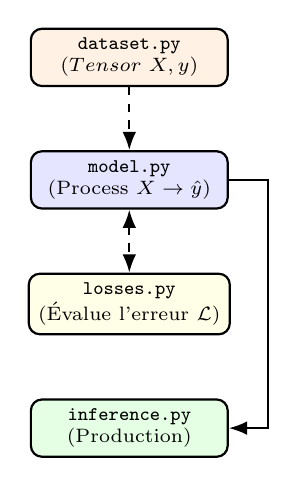
\begin{tikzpicture}[>=Latex, font=\scriptsize, box/.style={draw, rounded corners, thick, fill=white, align=center, minimum width=2.5cm, minimum height=0.6cm}]
\node[box, fill=orange!10] (data) {\texttt{dataset.py}\\($Tensor ~ X, y$)};
\node[box, fill=blue!10, below=0.8cm of data] (model) {\texttt{model.py}\\(Process $X \rightarrow \hat{y}$)};
\node[box, fill=yellow!10, below=0.8cm of model] (loss) {\texttt{losses.py}\\(Évalue l'erreur $\mathcal{L}$)};
\node[box, fill=green!10, below=0.8cm of loss] (infer) {\textbf{\texttt{inference.py}}\\(Production)};
\draw[->, thick, dashed] (data) -- (model);
\draw[<->, thick, dashed] (model) -- (loss);
\draw[->, thick] (model.east) -| ++(0.5,-1.6) |- (infer.east);
\end{tikzpicture}%
}{Interaction logique entre les fichiers source principaux}
\end{column}
\end{columns}
\end{frame}
\begin{frame}[t]{Implémentation — API REST locale}
\slidepurpose{Montrer comment le moteur d'inférence a été exposé à des clients externes sans casser l'interface web}{Architecture Logicielle}
\vspace*{-0.18cm}
\begin{columns}[T,onlytextwidth]
\begin{column}{0.56\textwidth}
\scriptsize
\setlength{\abovedisplayskip}{3pt}
\setlength{\belowdisplayskip}{3pt}
\begin{block}{Composants d'exposition}
\defitem{api.py}{Blueprint Flask sous \texttt{/api/v1} exposant \texttt{/health}, \texttt{/predict}, \texttt{/predict/gradcam} et \texttt{/benchmark}.}
\defitem{app.py}{Enregistre le Blueprint sans toucher aux routes HTML déjà utilisées par l'interface Flask.}
\defitem{service.py}{Conserve \texttt{model\_store} : le chargement du checkpoint reste \textbf{lazy} et partagé.}
\defitem{client.py}{CLI local pour tester l'API, afficher les métriques et exporter les images Grad-CAM.}
\end{block}
\begin{block}{Intérêt pratique}
\begin{itemize}
\setlength{\itemsep}{0.15em}
\item même moteur d'inférence pour le navigateur, \texttt{curl} et les scripts externes ;
\item point d'intégration propre pour une future interface plus riche ;
\item smoke tests simples via \texttt{/api/v1/health} et le client CLI.
\end{itemize}
\end{block}
\end{column}
\begin{column}{0.44\textwidth}
\begin{center}
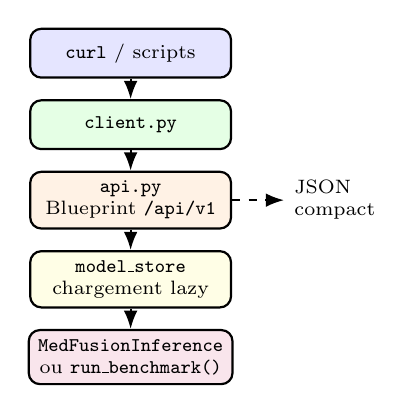
\begin{tikzpicture}[>=Latex, font=\scriptsize, box/.style={draw, rounded corners, thick, fill=white, align=center, minimum width=2.55cm, minimum height=0.62cm}]
\node[box, fill=blue!10] (curl) {\texttt{curl} / scripts};
\node[box, fill=green!10, below=0.26cm of curl] (client) {\texttt{client.py}};
\node[box, fill=orange!10, below=0.26cm of client] (api) {\texttt{api.py}\\Blueprint \texttt{/api/v1}};
\node[box, fill=yellow!10, below=0.26cm of api] (store) {\texttt{model\_store}\\chargement lazy};
\node[box, fill=purple!10, below=0.26cm of store] (infer) {\texttt{MedFusionInference}\\ou \texttt{run\_benchmark()}};
\draw[->, thick] (curl) -- (client);
\draw[->, thick] (client) -- (api);
\draw[->, thick] (api) -- (store);
\draw[->, thick] (store) -- (infer);
\draw[->, thick, dashed] (api.east) -- ++(0.66,0) node[right, align=left] {JSON\\compact};
\end{tikzpicture}
\end{center}
\end{column}
\end{columns}
\end{frame}
\begin{frame}[t]{Implémentation — Workflow d'une requête API}
\slidepurpose{Expliquer le cycle complet d'une requête, la validation de l'image et la structure des réponses JSON}{Déploiement local / intégration}
\vspace*{-0.18cm}
\begin{columns}[T,onlytextwidth]
\begin{column}{0.56\textwidth}
\scriptsize
\setlength{\abovedisplayskip}{3pt}
\setlength{\belowdisplayskip}{3pt}
\begin{block}{Cycle de traitement}
\begin{enumerate}
\setlength{\itemsep}{0.1em}
\item Entrée : \texttt{multipart/form-data} ou octets image bruts.
\item Validation : extension autorisée, ouverture PIL, conversion \texttt{RGB}.
\item Traitement : \texttt{engine.predict(...)} ou \texttt{run\_benchmark(max\_images)}.
\item Sortie : réponse \textbf{JSON} avec probabilités, métadonnées et temps d'inférence.
\end{enumerate}
\end{block}
\begin{block}{Choix d'implémentation}
\begin{itemize}
\setlength{\itemsep}{0.15em}
\item \texttt{/predict} : score simple, sans heatmap.
\item \texttt{/predict/gradcam} : overlay et heatmap en PNG Base64.
\item \texttt{/benchmark} : métriques seulement, graphes exclus.
\end{itemize}
\end{block}
\end{column}
\begin{column}{0.44\textwidth}
\scriptsize
\begin{block}{Routes exposées}
\begin{itemize}
\setlength{\itemsep}{0.1em}
\item \texttt{GET /api/v1/health}
\item \texttt{POST /api/v1/predict}
\item \texttt{POST /api/v1/predict/gradcam}
\item \texttt{GET /api/v1/benchmark?max\_images=20}
\end{itemize}
\end{block}
\begin{block}{Exemples d'appel}
\texttt{curl /api/v1/health}

\vspace{0.1cm}
\texttt{curl -X POST /api/v1/predict}

\vspace{0.03cm}
\texttt{-F "image=@radio.jpeg"}

\vspace{0.1cm}
\texttt{python client.py predict image.jpeg}

\vspace{0.03cm}
\texttt{--gradcam --save overlay.png}
\end{block}
\end{column}
\end{columns}
\end{frame}
\begin{frame}[t]{Implémentation — Exécution et Hyperparamètres}
\slidepurpose{Justifier les variables d'ajustement du code lors de l'apprentissage}{Lancement de l'Entraînement}
\vspace*{-0.18cm}
\begin{columns}[T,onlytextwidth]
\begin{column}{0.56\textwidth}
\footnotesize
\setlength{\abovedisplayskip}{3pt}
\setlength{\belowdisplayskip}{3pt}
\begin{block}{Lancement via \texttt{train.py}}
L'exécution de l'entraînement a été finement calibrée sur l'environnement Colab :
\begin{itemize}
\setlength{\itemsep}{0.15em}
\item \texttt{-\,-epochs 50} : Temps de chauffe suffisant pour stabiliser le réseau Transformer.
\item \texttt{-\,-batch\_size 16} : Contrainte optimale GPU allégeant la VRAM tout en maintenant le batch normalization fonctionnel.
\item \texttt{-\,-lr 1e-4} \& \textbf{AdamW} : Taux d'apprentissage modéré afin d'éviter l'oubli catastrophique du pré-entraînement CNN.
\end{itemize}
\end{block}
\end{column}
\begin{column}{0.44\textwidth}
\tikzsolutionfigure{%
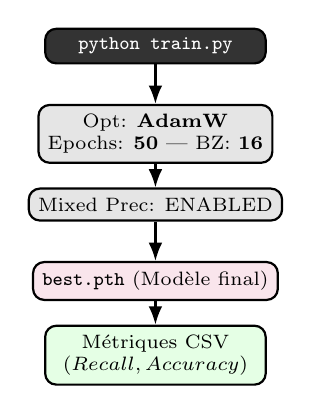
\begin{tikzpicture}[>=Latex, font=\scriptsize, box/.style={draw, rounded corners, thick, fill=white, align=center, minimum width=2.8cm}]
\node[box, fill=black!80, text=white] (train) {\texttt{python train.py}};
\node[box, fill=gray!20, below=0.5cm of train] (epoch) {Opt: \textbf{AdamW}\\Epochs: \textbf{50} | BZ: \textbf{16}};
\node[box, fill=gray!20, below=0.3cm of epoch] (amp) {Mixed Prec: ENABLED};
\node[box, fill=purple!10, below=0.5cm of amp] (out) {\texttt{best.pth} (Modèle final)};
\node[box, fill=green!10, below=0.3cm of out] (metrics) {Métriques CSV\\($Recall, Accuracy$)};
\draw[->, thick] (train) -- (epoch);
\draw[->, thick] (epoch) -- (amp);
\draw[->, thick] (amp) -- (out);
\draw[->, thick] (out) -- (metrics);
\end{tikzpicture}%
}{Flux d'exécution de l'entraînement et enregistrements}
\end{column}
\end{columns}
\end{frame}

\section{Résultats et Finalisation}

\begin{frame}{Résultats obtenus — synthèse quantitative}
\slidepurpose{Donner les performances finales du modèle sur le jeu de test et les interpréter}{Évaluation finale}
\footnotesize
\begin{columns}[T,onlytextwidth]
\begin{column}{0.53\textwidth}
\begin{block}{Protocole d'évaluation}
\begin{itemize}
\item \textbf{Jeu de test final :} 624 radiographies.
\item \textbf{Répartition :} 234 cas \texttt{NORMAL} et 390 cas \texttt{PNEUMONIA}.
\item \textbf{Checkpoint évalué :} \texttt{Model\_19Apr26.pth}.
\end{itemize}
\end{block}
\begin{block}{Indicateurs globaux}
\begin{itemize}
\item \textbf{Accuracy :} 92.79\%
\item \textbf{AUC-ROC :} 0.976
\item \textbf{Average Precision :} 0.984
\item \textbf{Erreurs totales :} 45 images sur 624 seulement
\end{itemize}
\end{block}
\end{column}
\begin{column}{0.45\textwidth}
\begin{block}{Classe \texttt{PNEUMONIA}}
\begin{itemize}
\item \textbf{Recall / Sensibilité :} 96.92\%
\item \textbf{Precision :} 91.97\%
\item \textbf{F1-score :} 94.38\%
\end{itemize}
\end{block}
\begin{block}{Classe \texttt{NORMAL}}
\begin{itemize}
\item \textbf{Recall / Spécificité :} 85.90\%
\item \textbf{Precision :} 94.37\%
\item \textbf{F1-score :} 89.93\%
\end{itemize}
\end{block}
\end{column}
\end{columns}
\end{frame}

\begin{frame}{Résultats obtenus — matrice de confusion et lecture métier}
\slidepurpose{Expliquer précisément où le modèle se trompe et pourquoi ces erreurs comptent}{Analyse détaillée des sorties}
\footnotesize
\begin{columns}[T,onlytextwidth]
\begin{column}{0.46\textwidth}
\begin{block}{Matrice de confusion}
\centering
\renewcommand{\arraystretch}{1.25}
\resizebox{0.98\linewidth}{!}{%
\begin{tabular}{|c|c|c|}
\hline
\textbf{Vrai / Prédit} & \textbf{NORMAL} & \textbf{PNEUMONIA} \\
\hline
\textbf{NORMAL} & 201 & 33 \\
\hline
\textbf{PNEUMONIA} & 12 & 378 \\
\hline
\end{tabular}
}
\end{block}
\begin{block}{Bilan chiffré}
\begin{itemize}
\item \textbf{Vrais positifs :} 378
\item \textbf{Vrais négatifs :} 201
\item \textbf{Faux positifs :} 33
\item \textbf{Faux négatifs :} 12
\end{itemize}
\end{block}
\end{column}
\begin{column}{0.50\textwidth}
\begin{block}{Interprétation}
\begin{itemize}
\item Sur \textbf{390} cas de pneumonie, le système en détecte \textbf{378}.
\item Le taux de cas pneumonie manqués est de \textbf{12 / 390 = 3.08\%}.
\item Sur \textbf{234} images normales, \textbf{33} sont surclassées à tort en pneumonie.
\item Le modèle est donc \textbf{volontairement plus sensible que spécifique} : il déclenche plus facilement une alerte plutôt que de laisser passer une pneumonie.
\item En contexte de triage, ce compromis reste \textbf{cohérent médicalement}.
\end{itemize}
\end{block}
\end{column}
\end{columns}
\end{frame}

\begin{frame}{Résultats obtenus — benchmark visuel sur le jeu de test}
\slidepurpose{Montrer visuellement la qualité de séparation du modèle à l'échelle du test complet}{Benchmark final}
\scriptsize
\begin{columns}[T,onlytextwidth]
\begin{column}{0.68\textwidth}
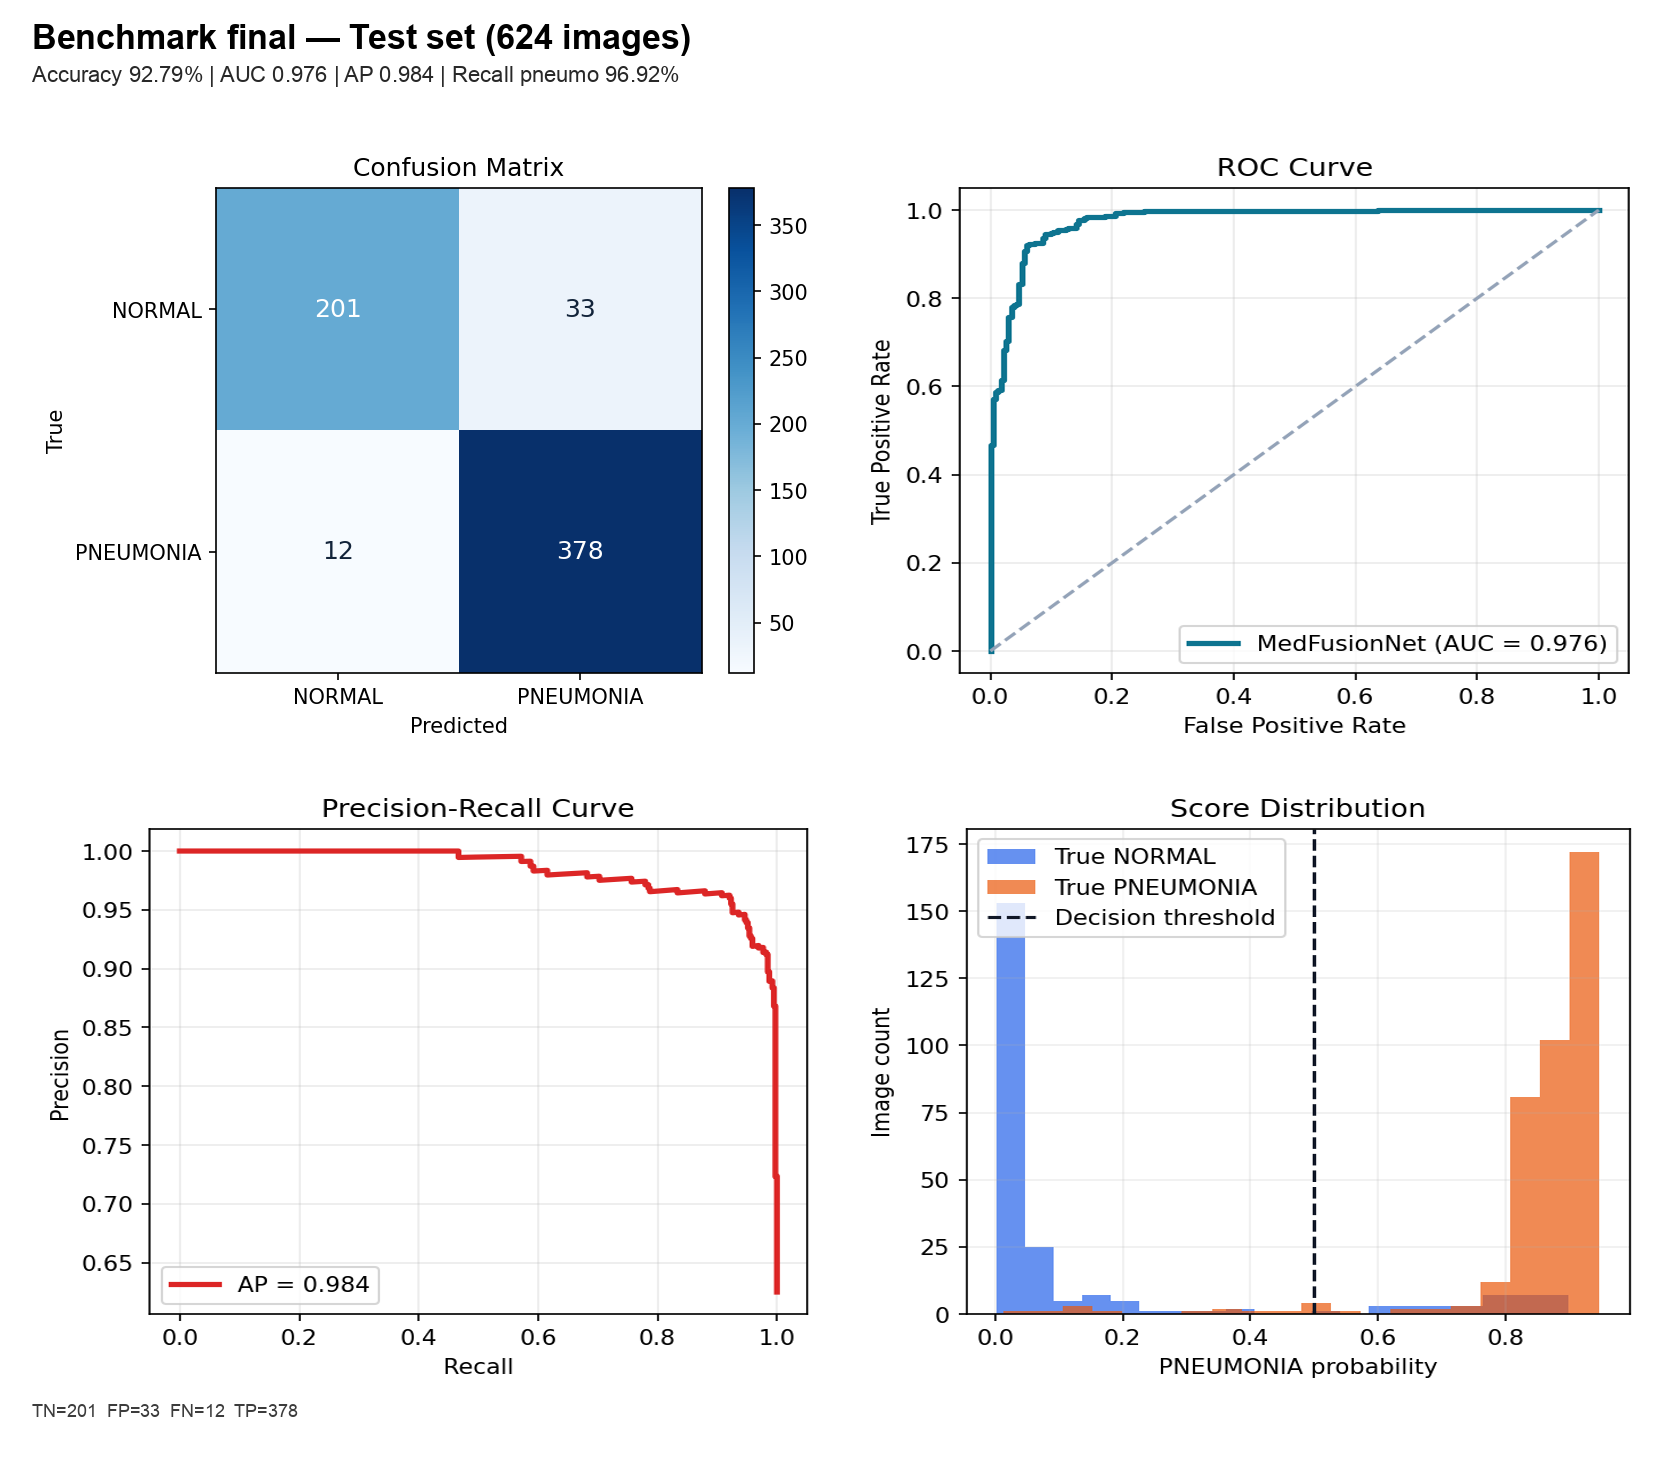
\includegraphics[width=\linewidth,height=0.74\textheight,keepaspectratio]{benchmark_testset.png}
\end{column}
\begin{column}{0.29\textwidth}
\begin{block}{Ce que montrent les courbes}
\begin{itemize}
\item \textbf{ROC :} courbe très proche du coin supérieur gauche.
\item \textbf{PR :} AP = \textbf{0.984}, donc très bon classement des cas pneumonie.
\item Les scores sont \textbf{bien séparés} ; peu d'ambiguïté autour du seuil 0.5.
\end{itemize}
\end{block}
\end{column}
\end{columns}
\end{frame}

\begin{frame}{Résultats obtenus — comportement durant l'entraînement}
\slidepurpose{Lire les courbes d'apprentissage et signaler les limites de validation}{Analyse du run conservé}
\scriptsize
\begin{columns}[T,onlytextwidth]
\begin{column}{0.70\textwidth}
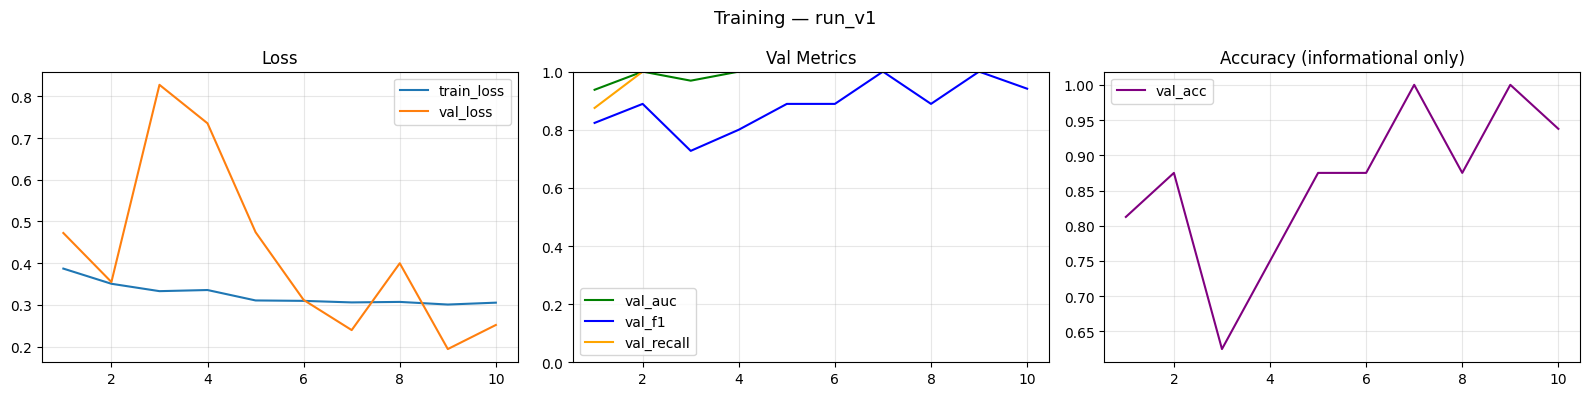
\includegraphics[width=\linewidth,height=0.71\textheight,keepaspectratio]{benchmark_training.png}
\end{column}
\begin{column}{0.27\textwidth}
\begin{block}{Lecture des courbes}
\begin{itemize}
\item La \textbf{train loss} baisse régulièrement : le modèle apprend effectivement.
\item La \textbf{val loss} oscille davantage : la validation est plus instable.
\item Les métriques montent vite, mais la validation ne contient que \textbf{16 images}.
\item La conclusion finale doit donc s'appuyer sur le \textbf{test set à 624 images}.
\end{itemize}
\end{block}
\end{column}
\end{columns}
\end{frame}

\begin{frame}{Résultats obtenus — validation qualitative par Grad-CAM}
\slidepurpose{Montrer comment l'explicabilité visuelle aide à valider le comportement du modèle}{Interprétabilité}
\footnotesize
\begin{columns}[T,onlytextwidth]
\begin{column}{0.66\textwidth}
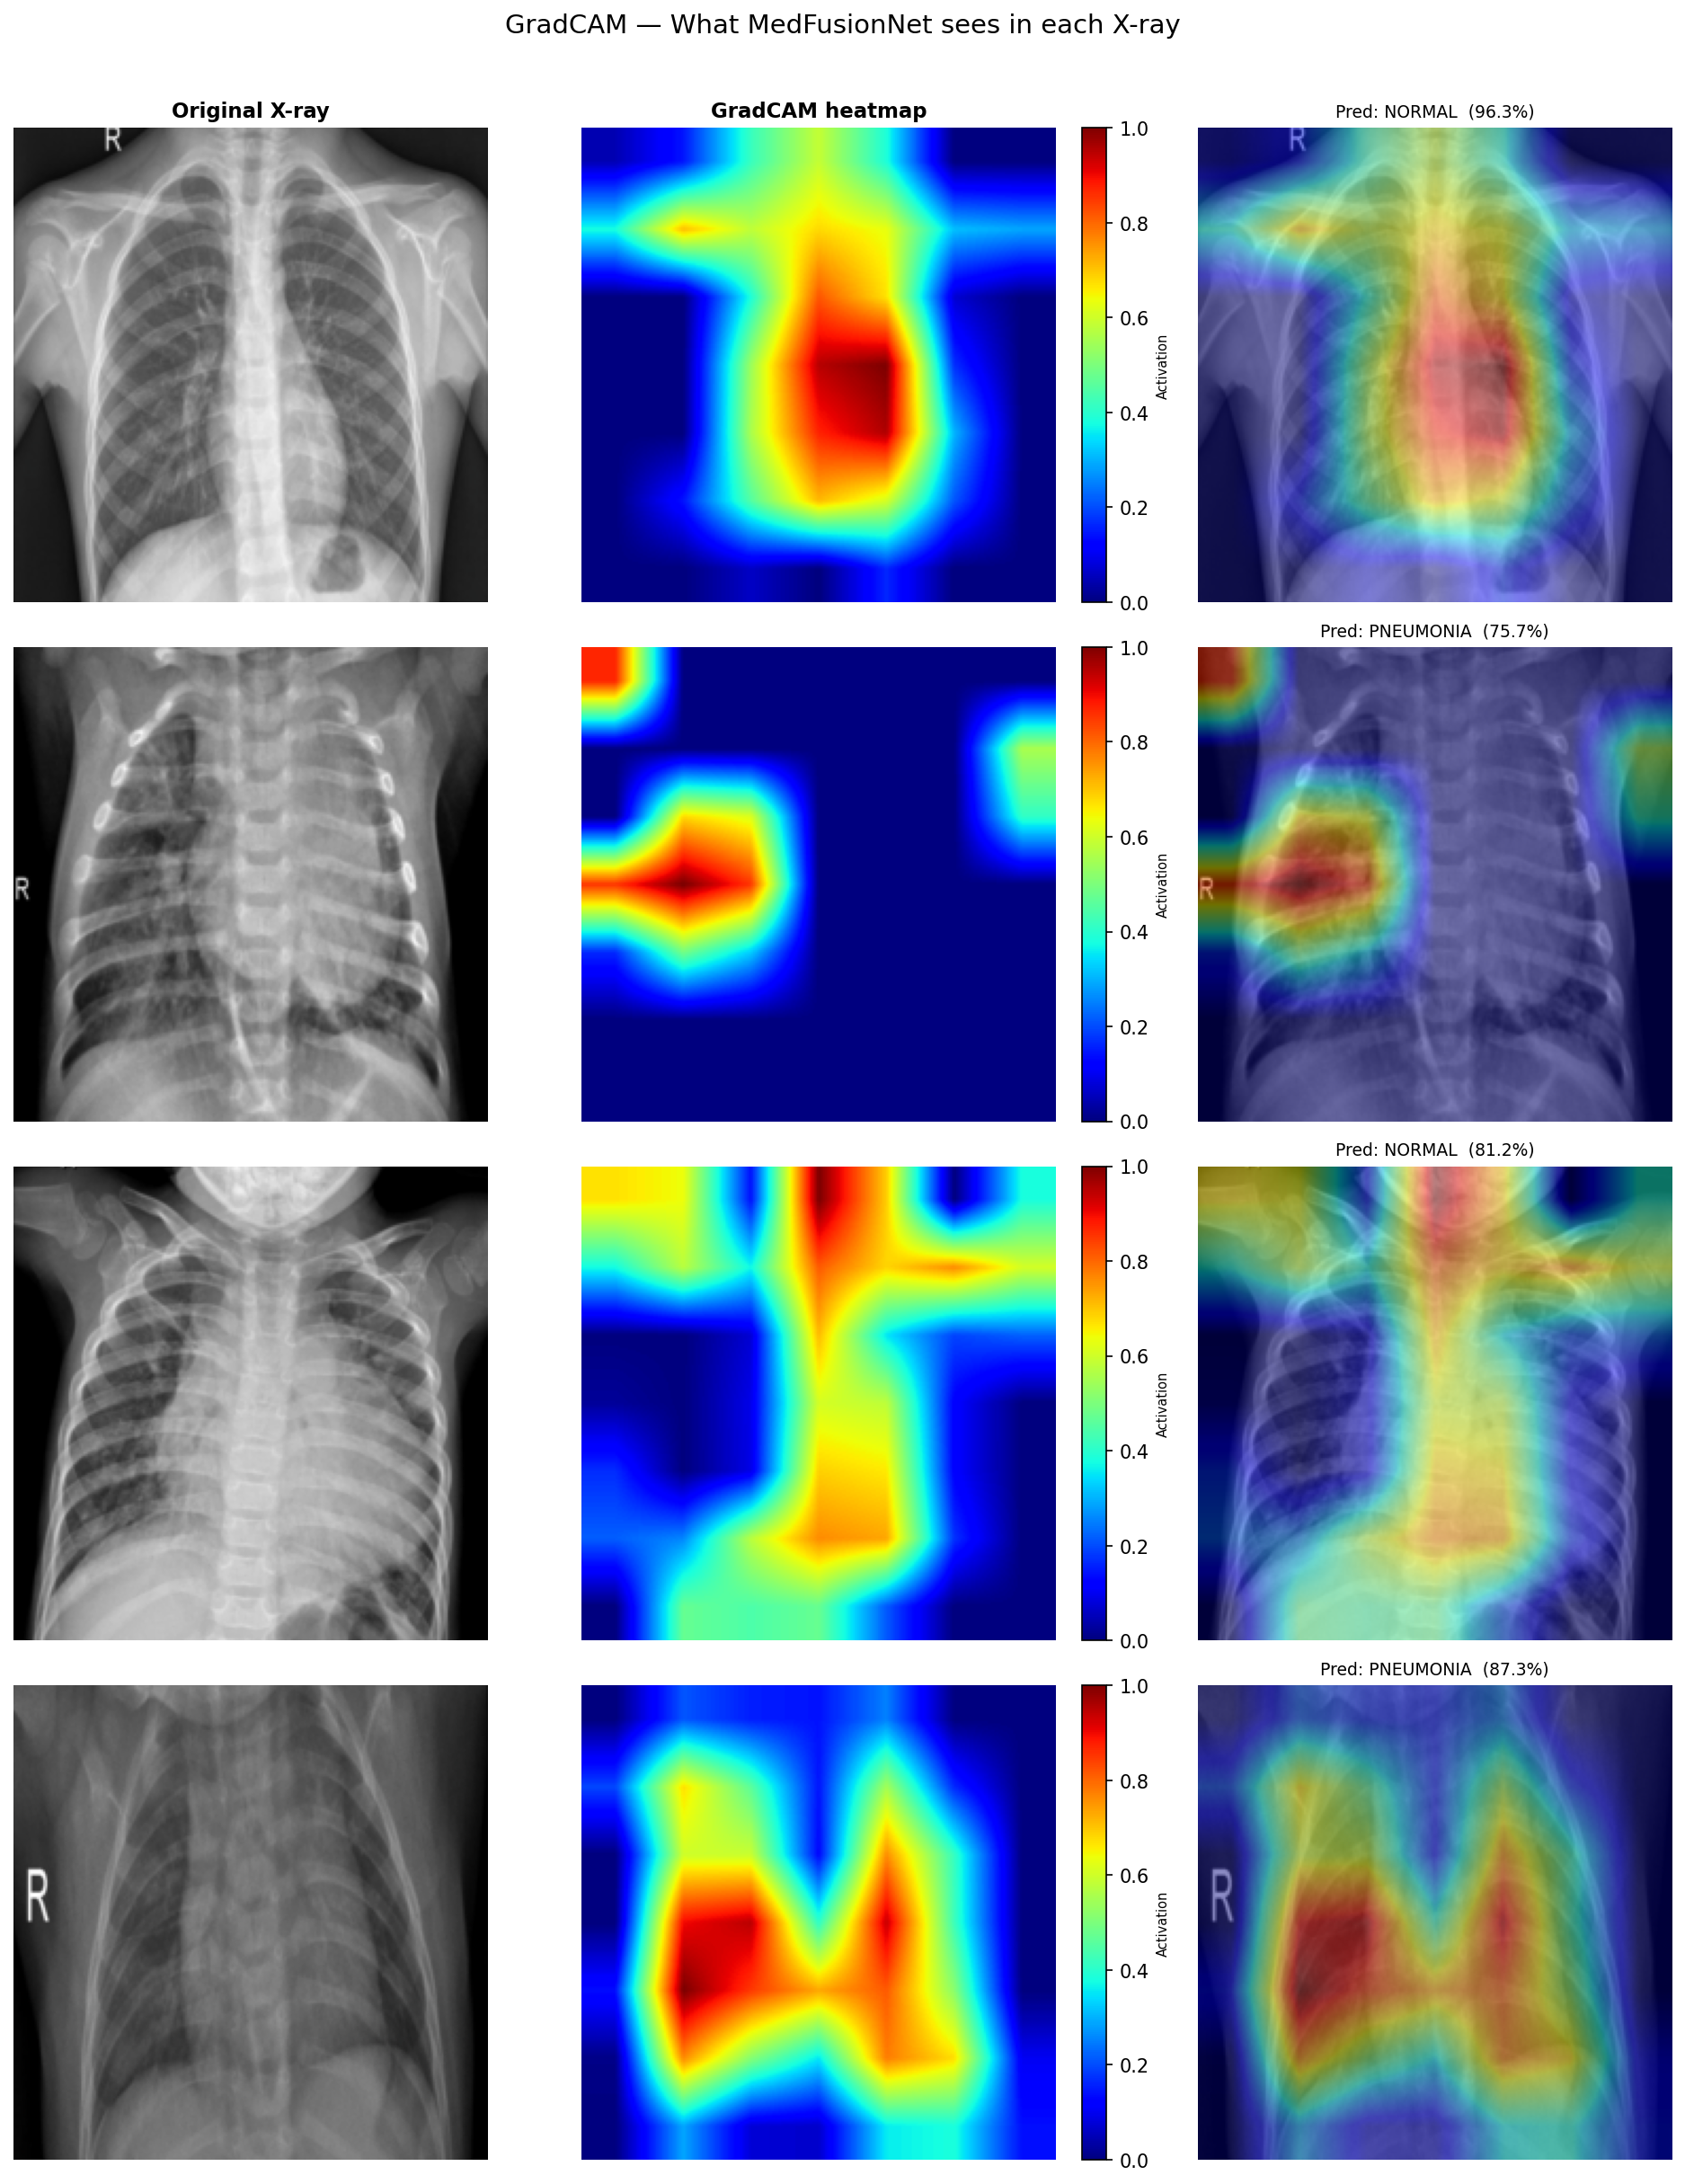
\includegraphics[width=\linewidth,height=0.73\textheight,keepaspectratio]{gradcam_results.png}
\end{column}
\begin{column}{0.31\textwidth}
\begin{block}{Ce que l'on observe}
\begin{itemize}
\item Les activations se concentrent surtout sur les \textbf{champs pulmonaires} et sur des zones cohérentes avec des opacités.
\item Le modèle ne semble pas décider uniquement à partir des bords ou du fond de l'image.
\item Grad-CAM aide à expliquer \textbf{où} le réseau regarde, mais reste un \textbf{outil qualitatif}.
\end{itemize}
\end{block}
\end{column}
\end{columns}
\end{frame}

\begin{frame}{Finalisation du projet}
\slidepurpose{Résumer les livrables concrets du projet et la suite logique}{Clôture / mise en production locale}
\scriptsize
\begin{columns}[T,onlytextwidth]
\begin{column}{0.49\textwidth}
\begin{block}{Livrables finalisés}
\begin{itemize}
\item \textbf{Modèle final entraîné} et checkpoint exporté.
\item \textbf{Runtime Python} modulaire avec CLI et API locale.
\item \textbf{Interface web Flask} pour charger une image, lancer l'inférence et voir le Grad-CAM.
\item \textbf{Benchmark local} avec ROC, PR, matrice de confusion et distribution des scores.
\end{itemize}
\end{block}
\end{column}
\begin{column}{0.47\textwidth}
\begin{block}{Conclusion technique}
\begin{itemize}
\item Le système est \textbf{fonctionnel de bout en bout}.
\item Les performances sont \textbf{suffisamment fortes} pour démontrer la viabilité de l'approche hybride Swin + DenseNet.
\item Le compromis retenu favorise la \textbf{détection des cas positifs}, ce qui est cohérent avec l'objectif médical.
\end{itemize}
\end{block}
\begin{block}{Améliorations futures}
\begin{itemize}
\item augmenter la taille du jeu de validation
\item renforcer la spécificité
\item tester sur un dataset externe et améliorer la calibration
\end{itemize}
\end{block}
\end{column}
\end{columns}
\end{frame}
\end{document}
